\section{Results and Discussion}
\label{ch3:sec:results}

\subsection{Algorithm performance for synchronised operation}
\label{ch3:subsec:algorithm-performance-synchronised}

The objective of the smart-charging algorithm is to distribute the charging demand of a fleet of EVs over the underlying base demand in such a way that no additional demand spikes are produced.
After assigning each EV's energy demand to its initially known demand trough, the algorithm produces a new demand spike since all EVs are charging simultaneously.
Through repetitive iterations and reallocating a portion of the assigned energy to different demand troughs, the algorithm is then able to spread all EVs' demands to form a flat demand profile in the end.
This process is shown in Figure~\ref{ch3:fig:time-series}.

\begin{figure}\centering
	\subfloat[]{
		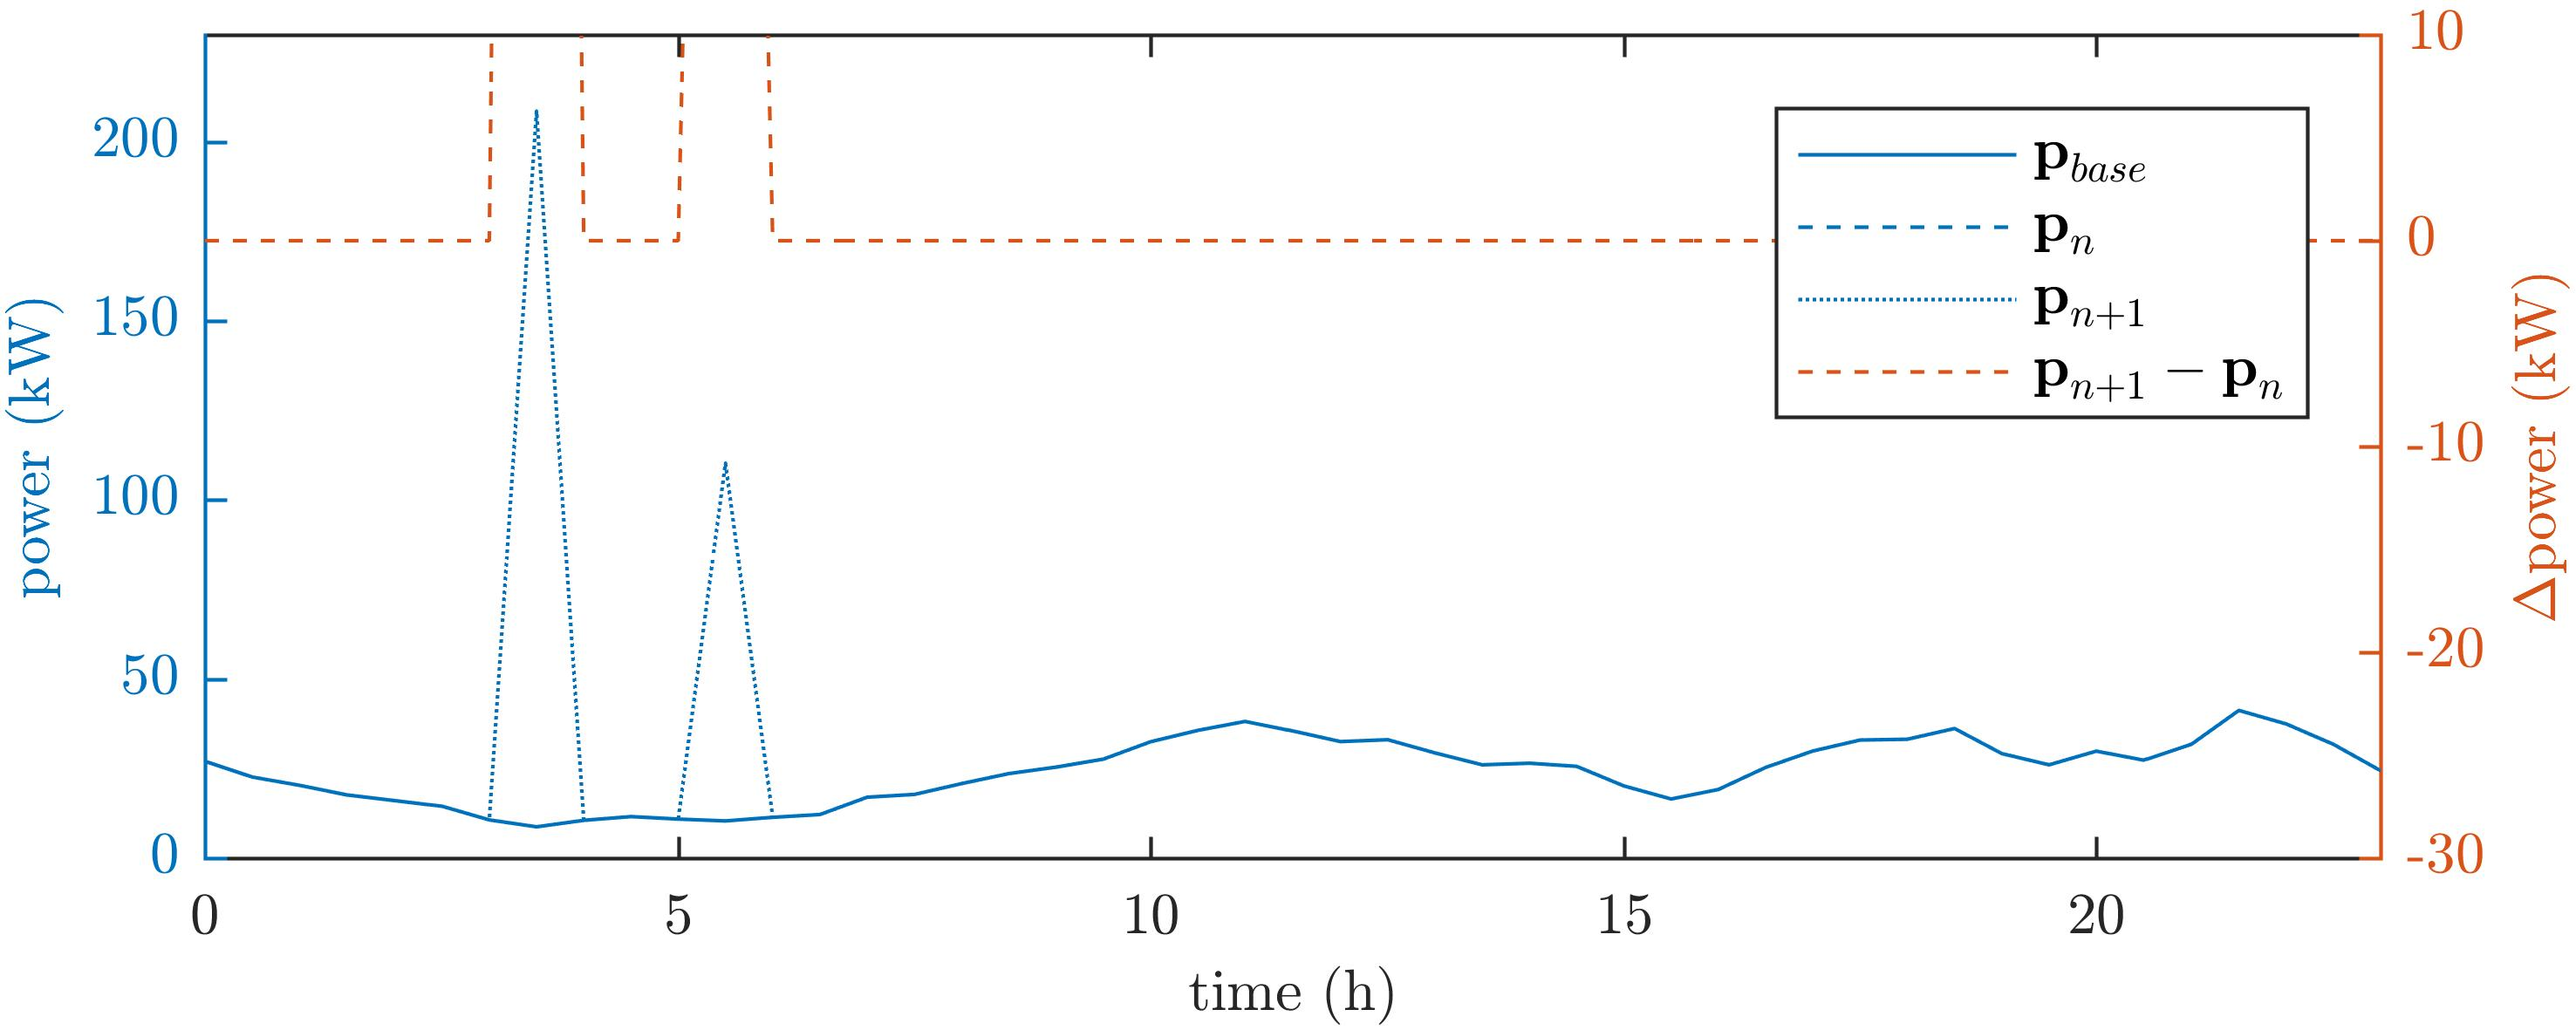
\includegraphics[height=4.5cm]{_chapter3/fig/time-series/ts-i0001}
		\label{ch3:subfig:time-series-1}
	}\\
	\subfloat[]{
		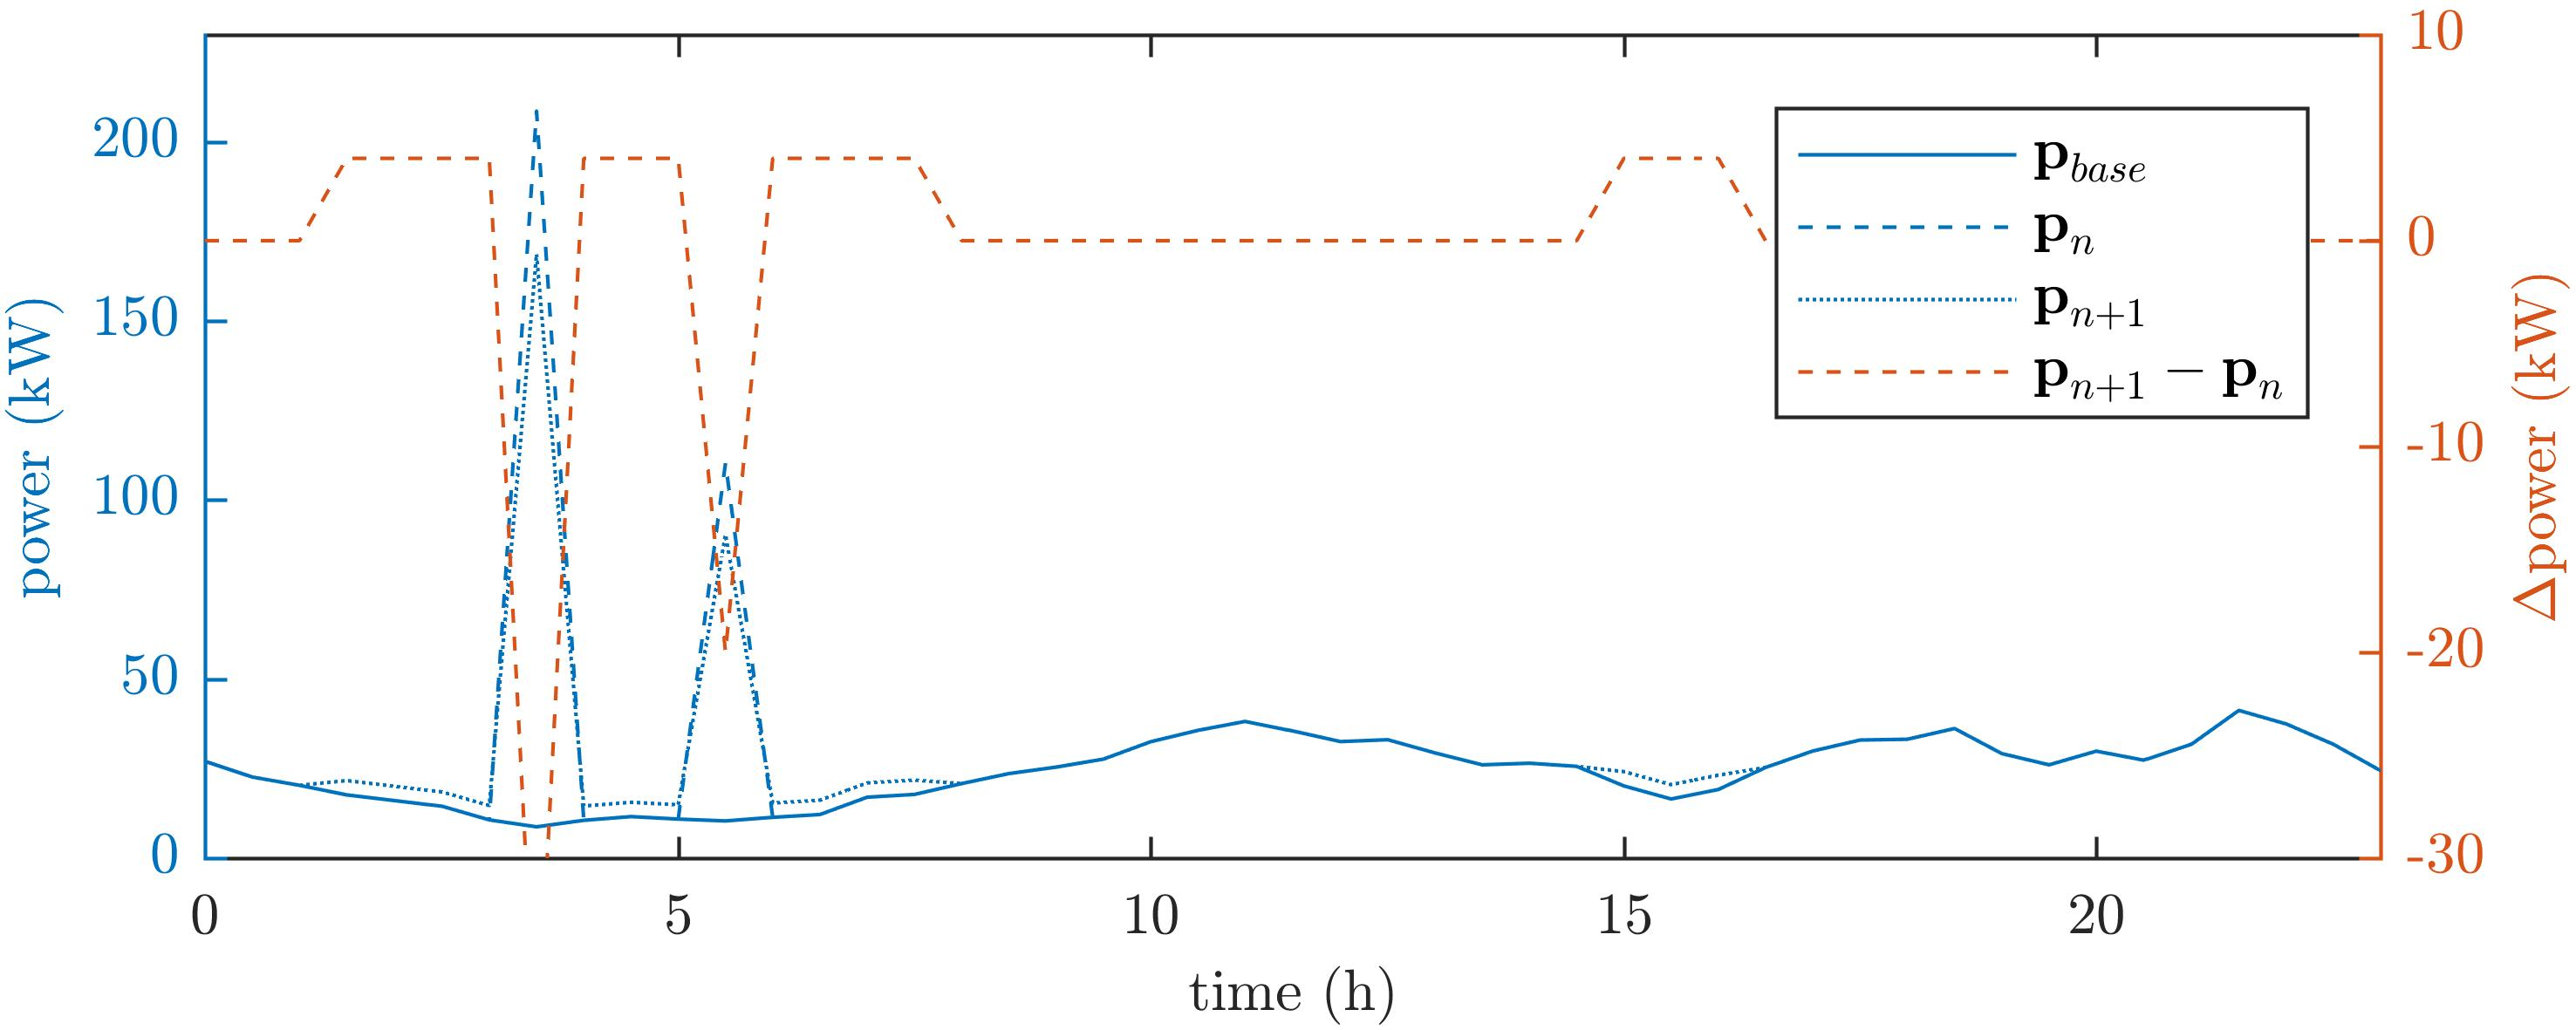
\includegraphics[height=4.5cm]{_chapter3/fig/time-series/ts-i0002}
		\label{ch3:subfig:time-series-2}
	}\\
	\subfloat[]{
		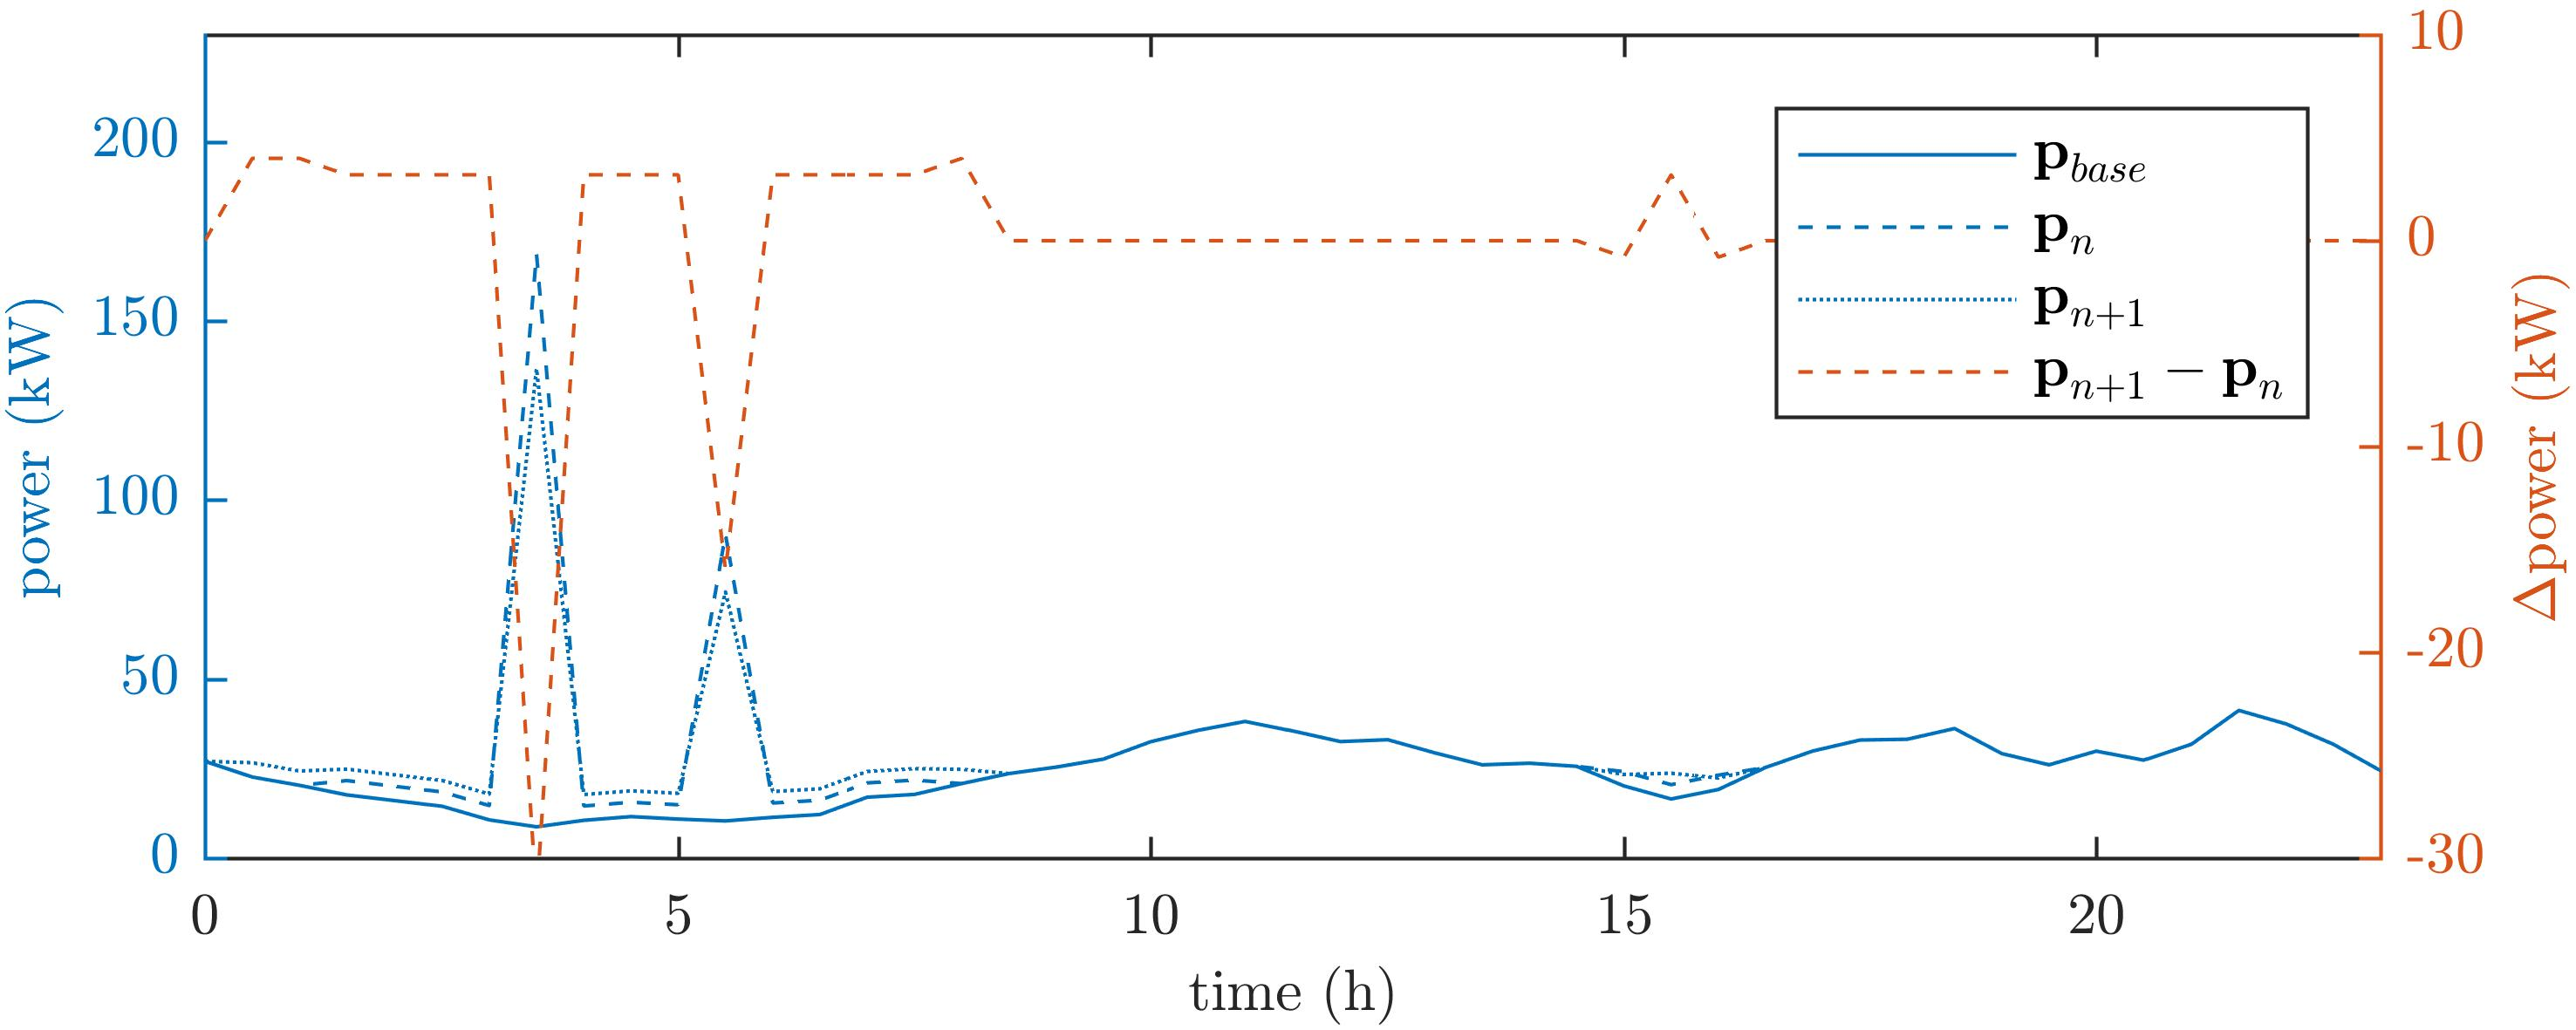
\includegraphics[height=4.5cm]{_chapter3/fig/time-series/ts-i0003}
		\label{ch3:subfig:time-series-3}
	}\\
	\subfloat[]{
		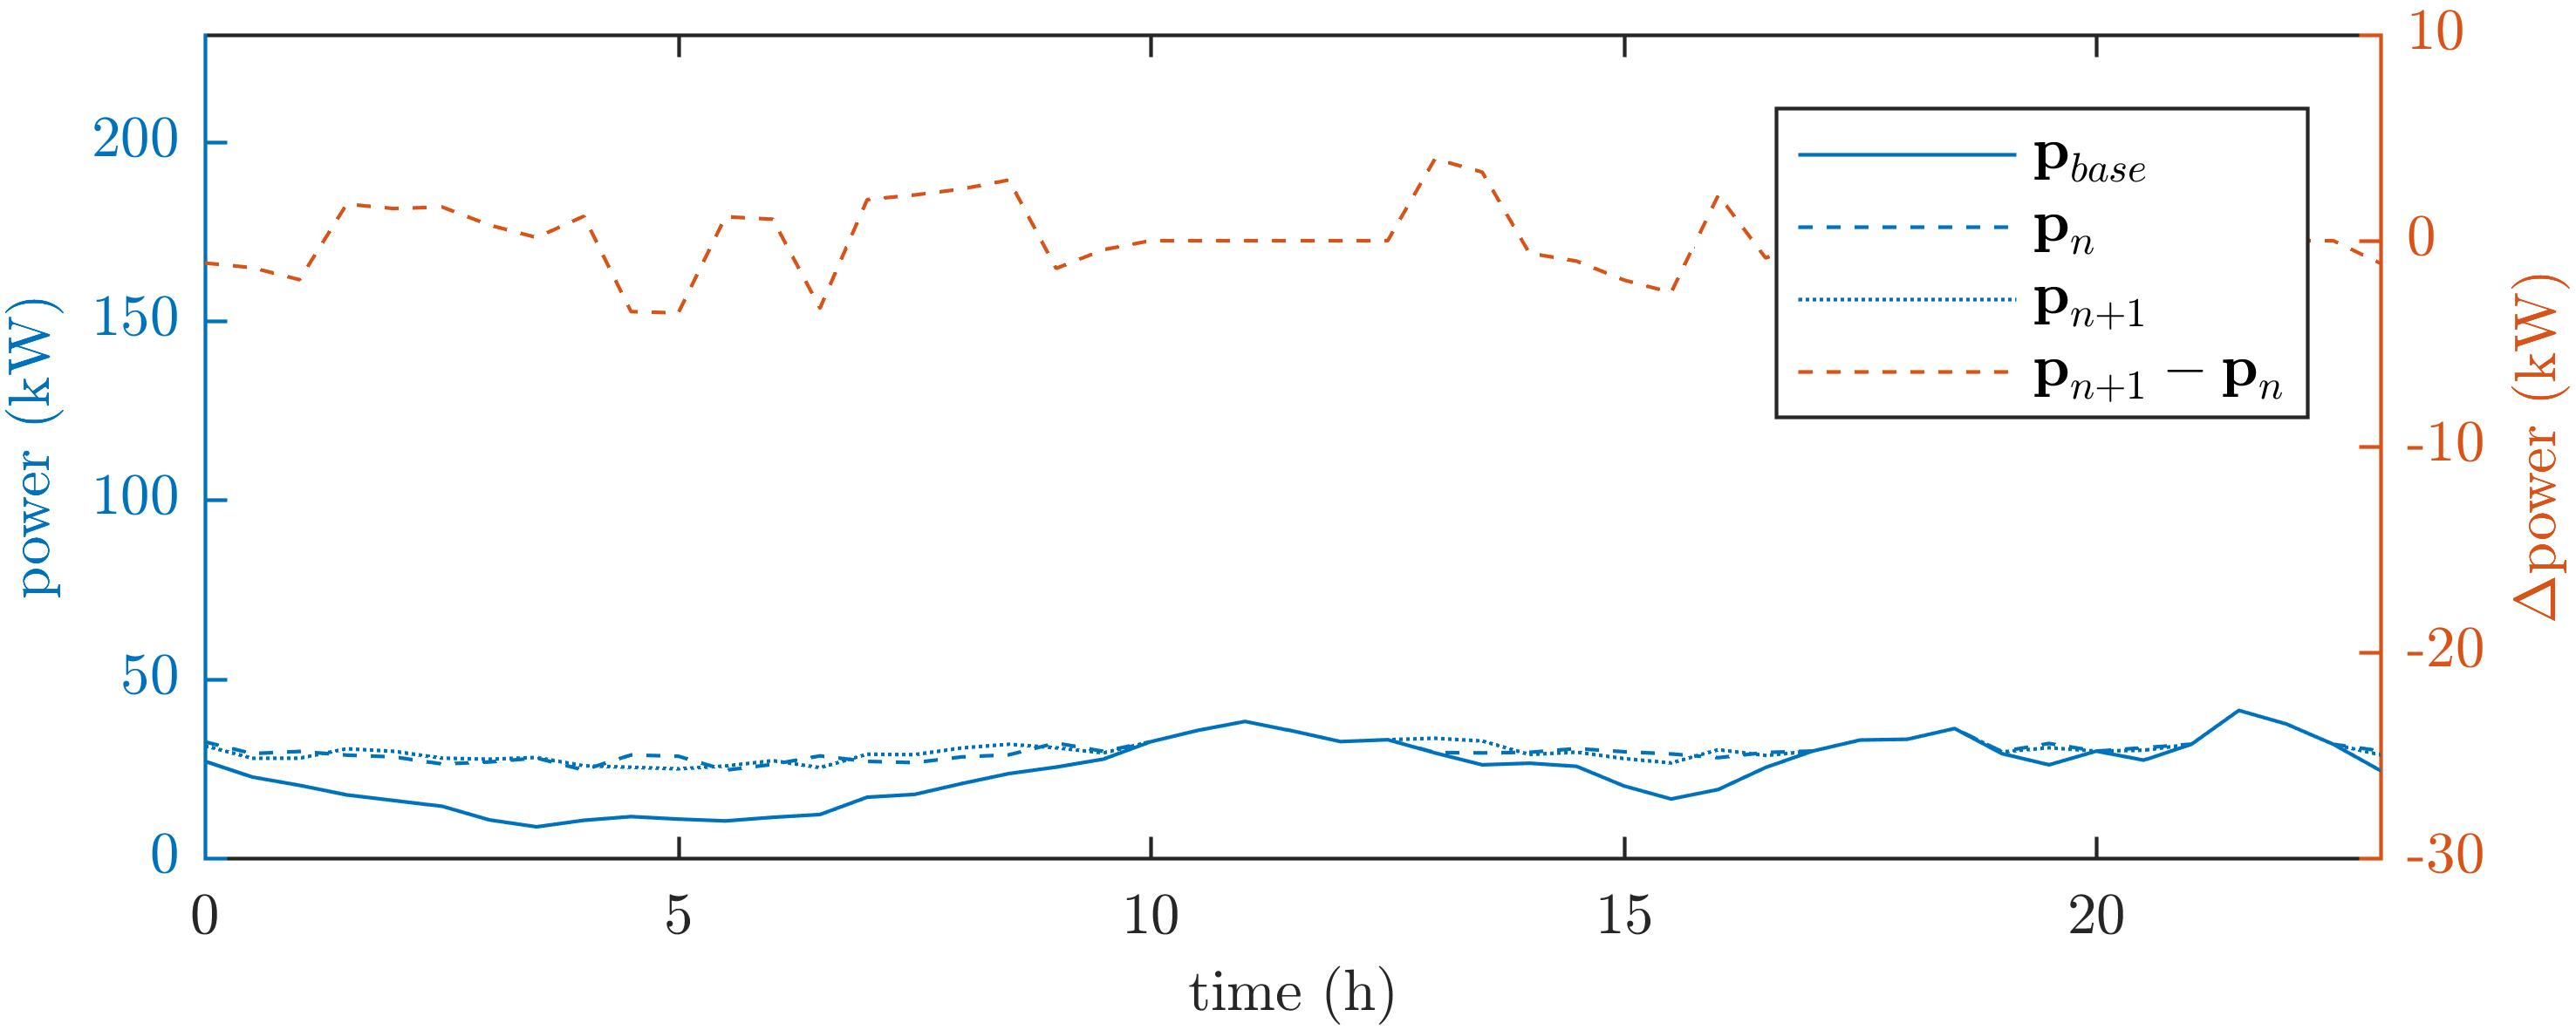
\includegraphics[height=4.5cm]{_chapter3/fig/time-series/ts-i0100}
		\label{ch3:subfig:time-series-last}
	}
\caption{Time series evolution for $\alpha=0.02$ and $\beta=0.20$, where (a) is at $n=1$, (b) is at $n=2$, (c) is at $n=3$, and (d) is at $n=N-1$.}
\label{ch3:fig:time-series}
\end{figure}

Here, the first algorithm iteration is shown in Figure~\ref{ch3:subfig:time-series-1}, where allocated power profile produces two new morning spikes of around 200kW and subsequently 110kW.
The second iteration however reduces these spikes by the factor $\alpha$ (i.e $0.2$) and redistributes the undone charging powers over the new power profile.
Figure~\ref{ch3:subfig:time-series-2} shows this reduction and reallocation.
Figure~\ref{ch3:subfig:time-series-3} is the third iteration that reduces and redistributes the peaks even further.
In the end, i.e. when $n=N$, the resulting power profile becomes as flat as possible, which is shown in Figure~\ref{ch3:subfig:time-series-last}.
Throughout these iterations, it can be observed how the peak load in the total power, i.e. $\textbf{p}_n$, reduces and it can be observed how the changes in charging power, i.e. $\textbf{p}_{n+1}-\textbf{p}_n$, reduce in variance, which indicates that the algorithm works for the chosen parameters of $\alpha$ and $\beta$.
However, different parameters of $\alpha$ and $\beta$ do impact the performance of this synchronised algorithm execution, as shown in Figure~\ref{ch3:fig:oscillation}.

\begin{figure}\centering
	\subfloat[]{
		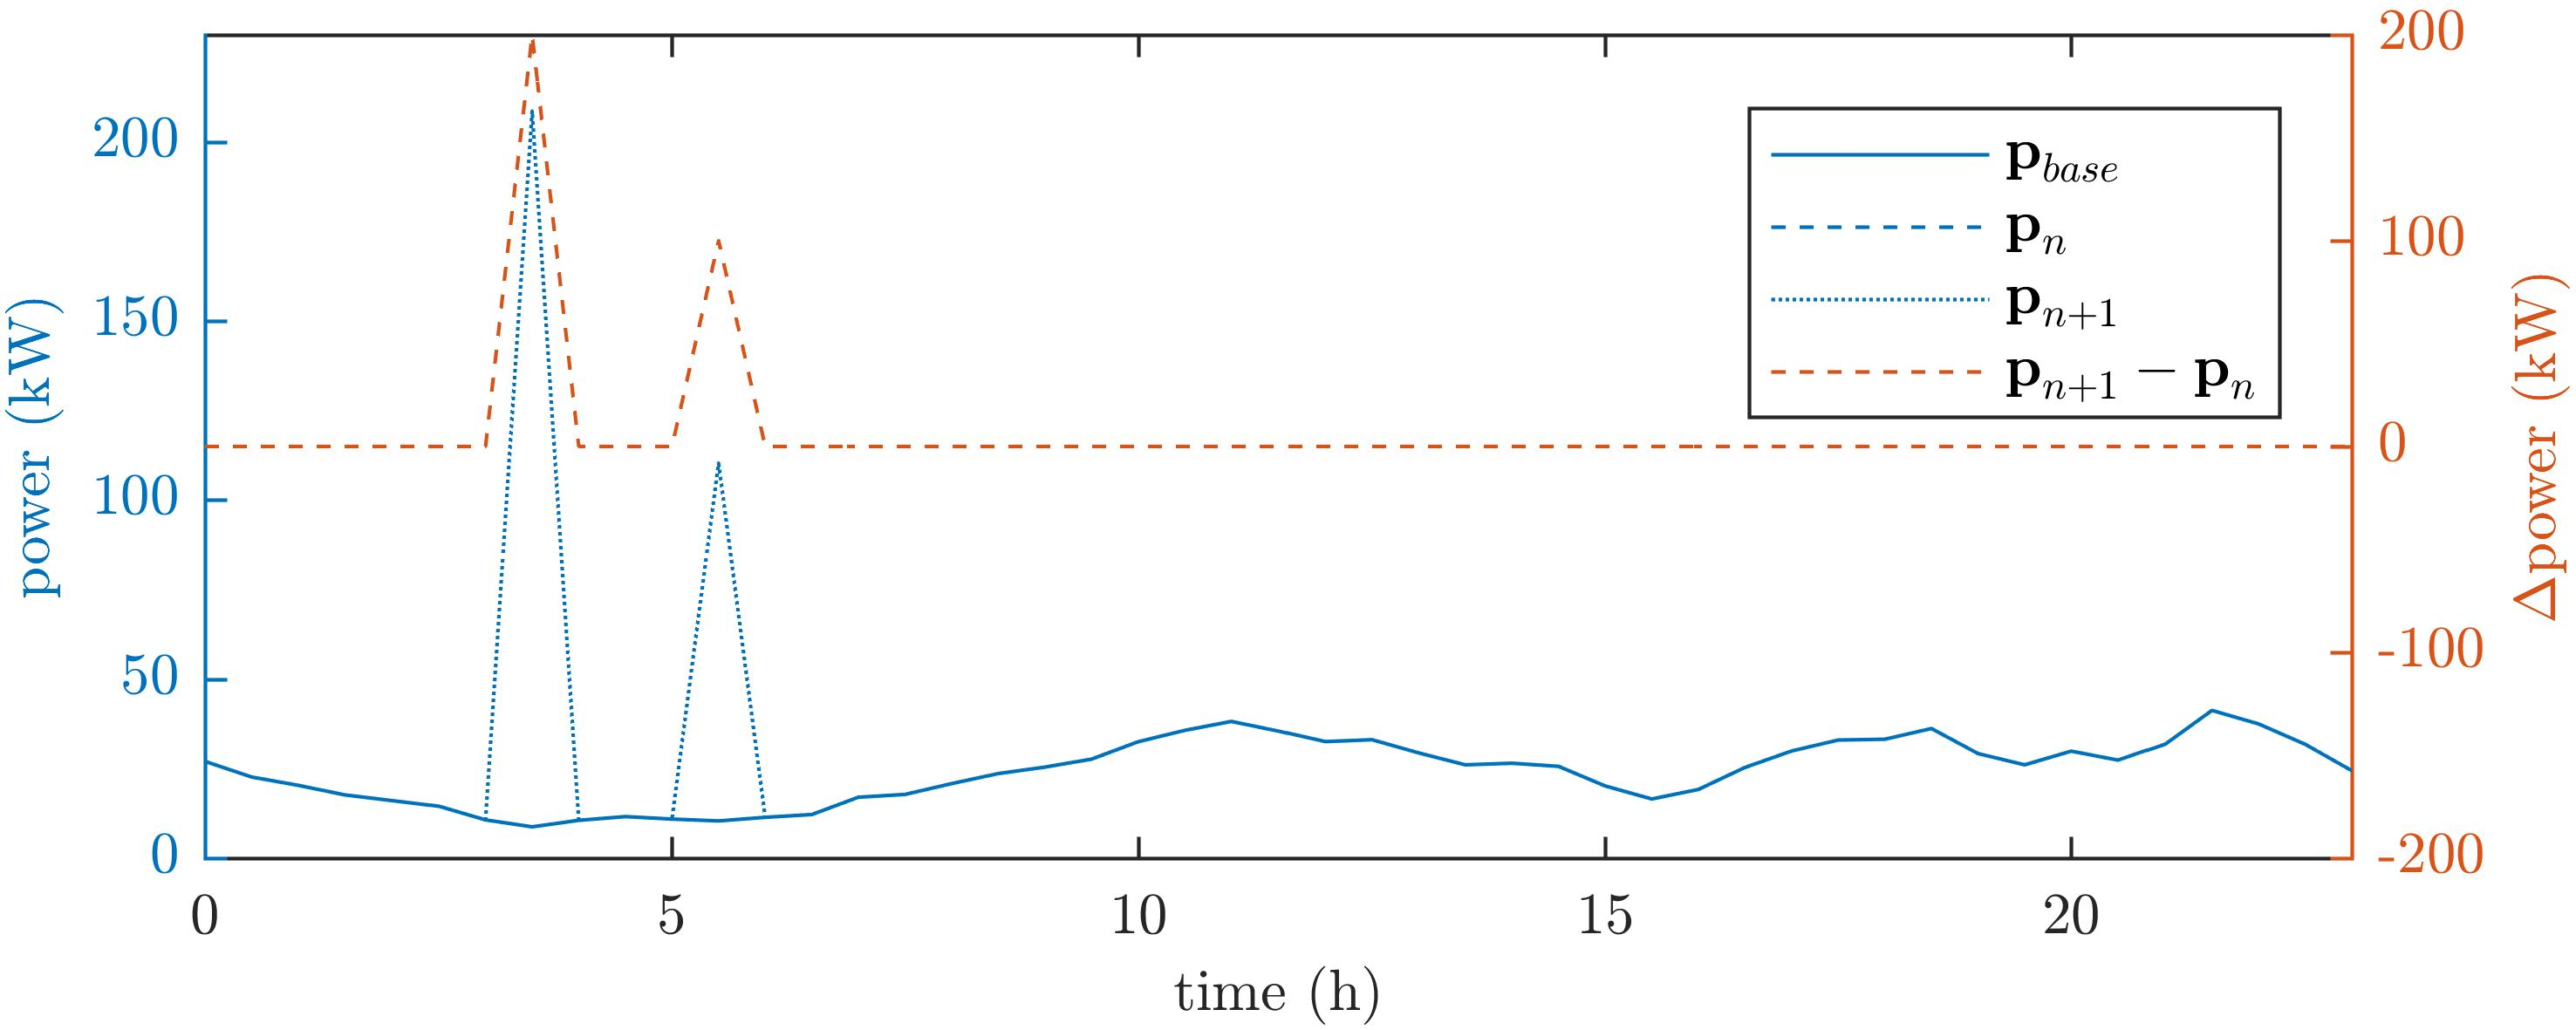
\includegraphics[height=4.5cm]{_chapter3/fig/oscillation/ts-i0001}
		\label{ch3:subfig:oscillation-1}
	}\\
	\subfloat[]{
		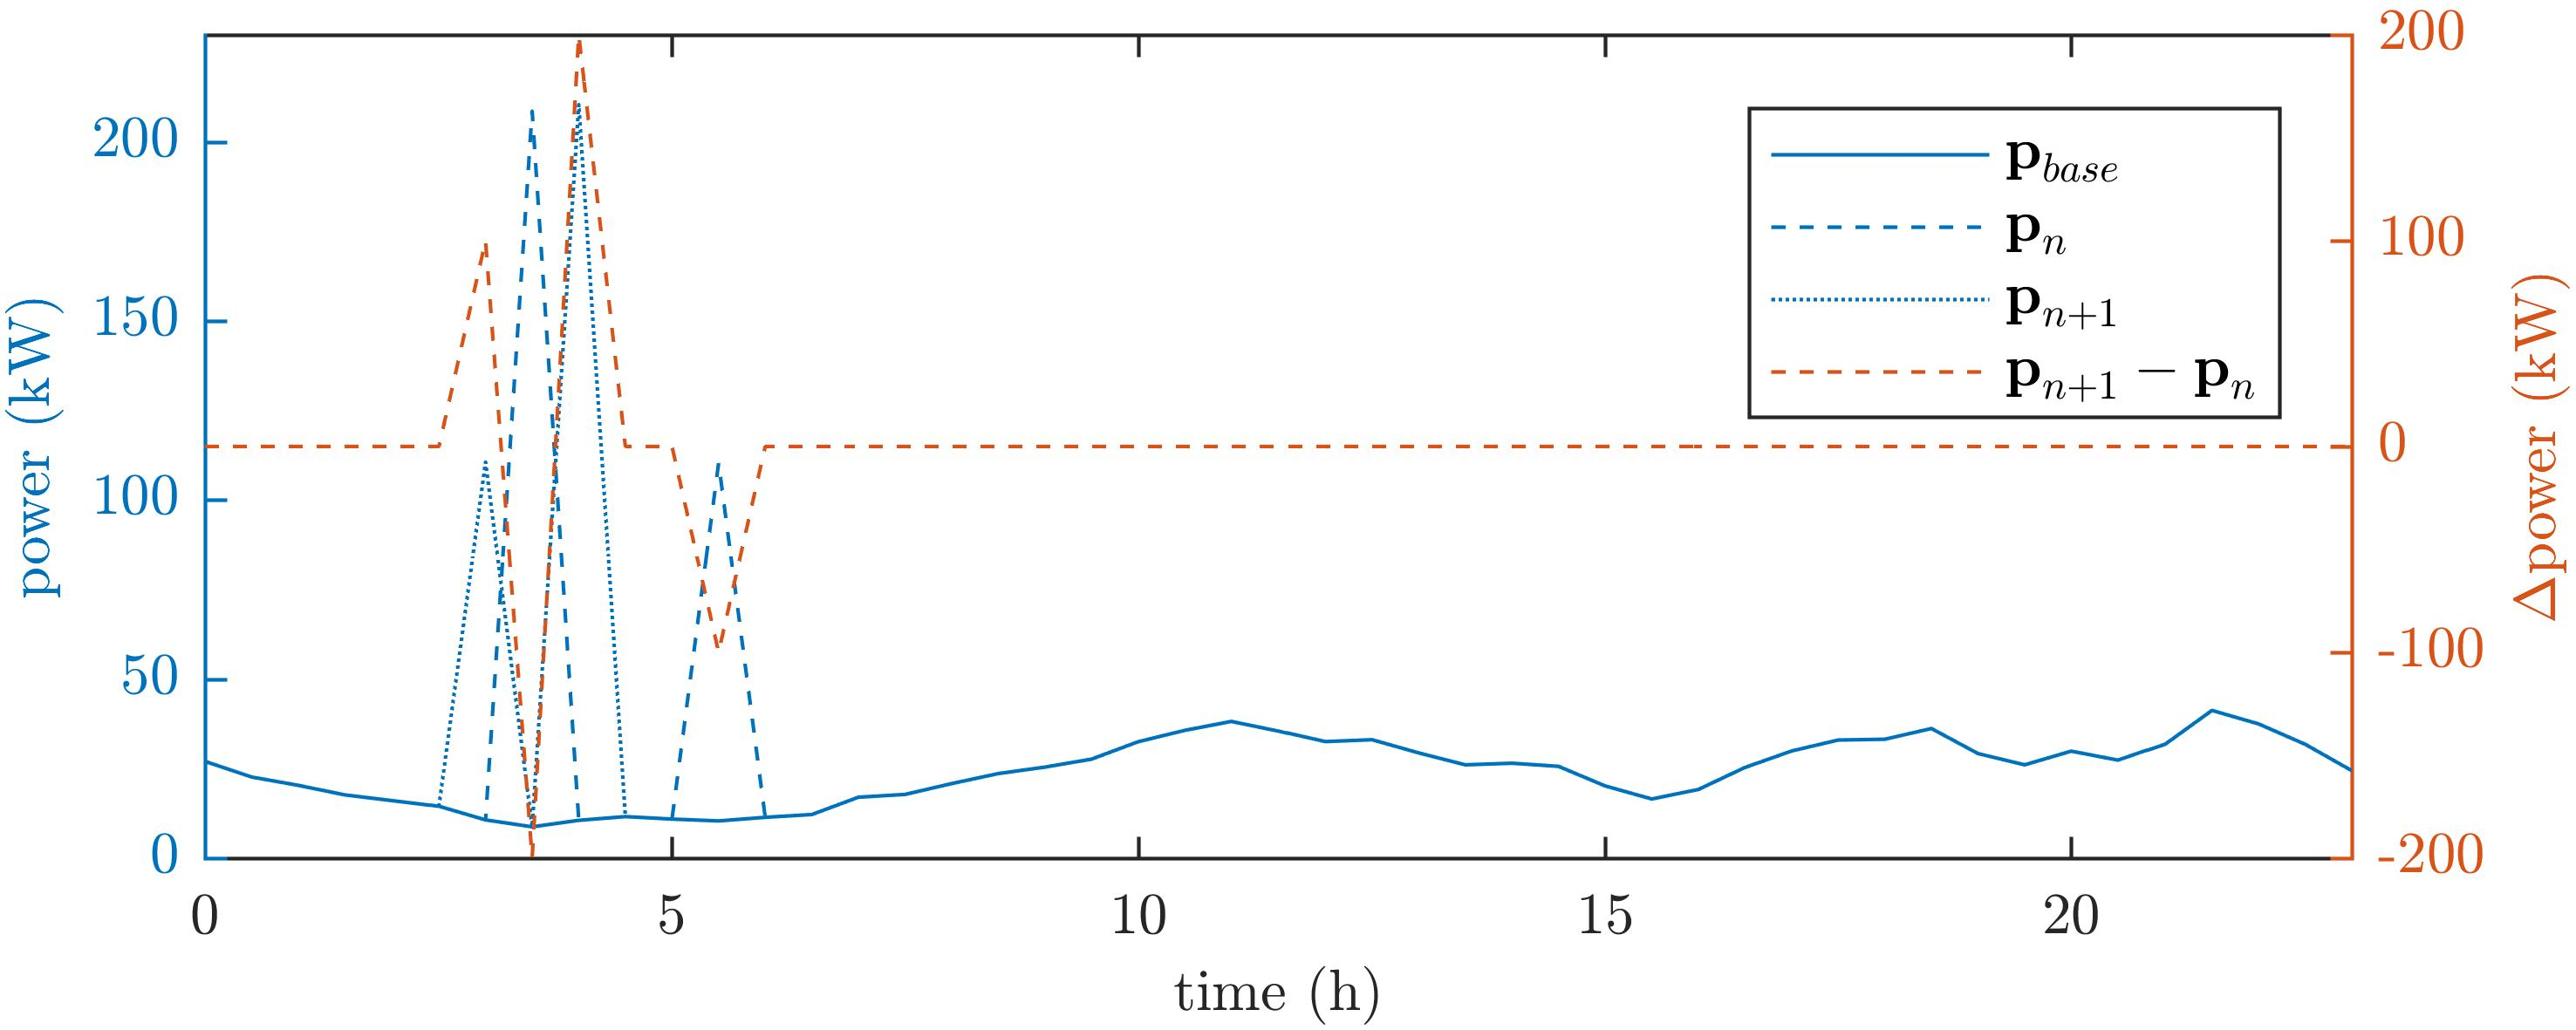
\includegraphics[height=4.5cm]{_chapter3/fig/oscillation/ts-i0002}
		\label{ch3:subfig:oscillation-2}
	}\\
	\subfloat[]{
		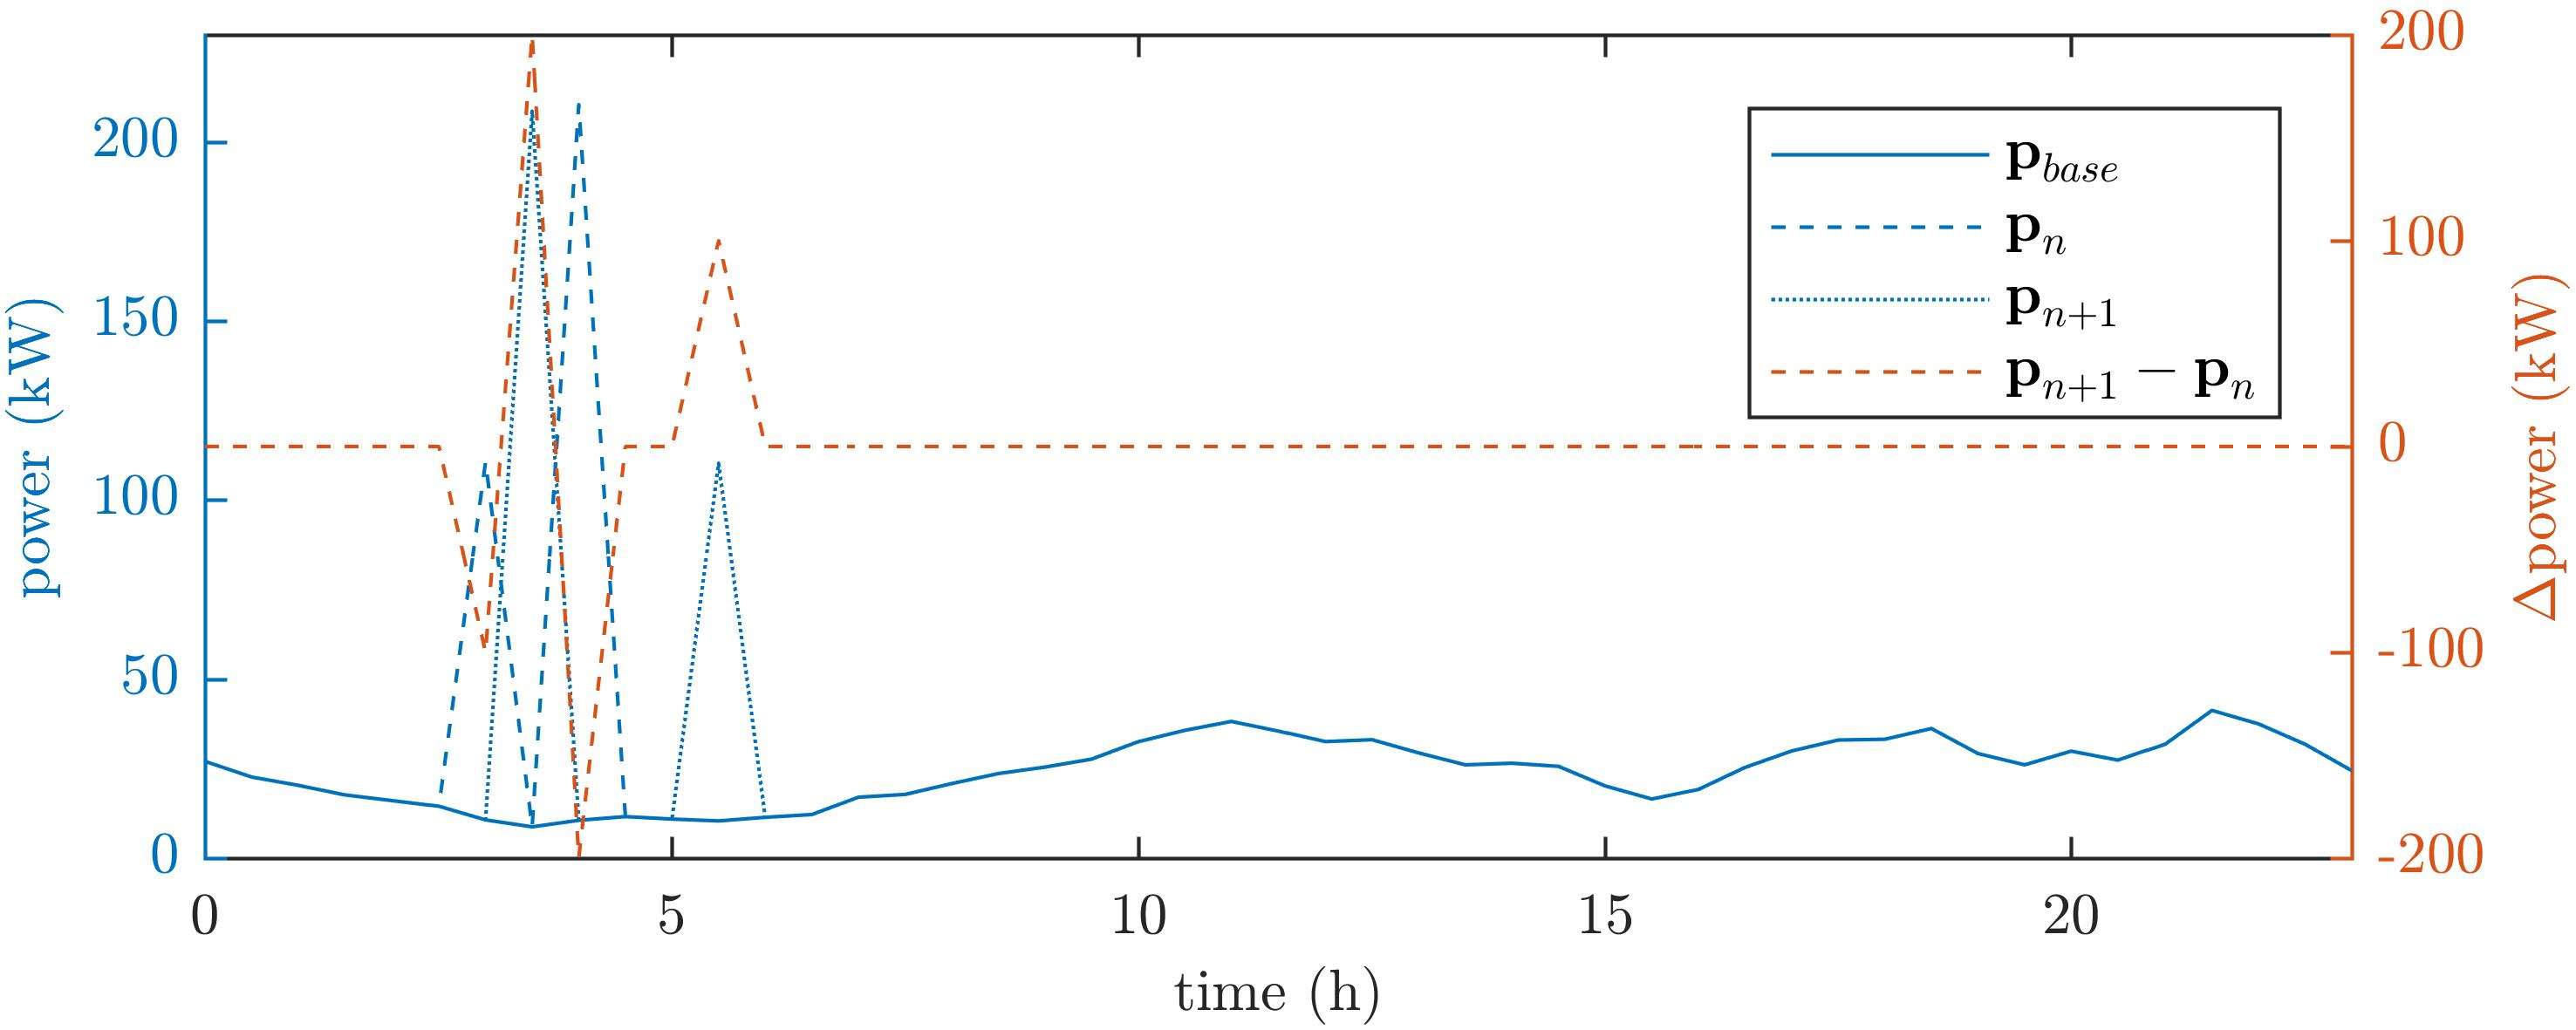
\includegraphics[height=4.5cm]{_chapter3/fig/oscillation/ts-i0003}
		\label{ch3:subfig:oscillation-3}
	}\\
	\subfloat[]{
		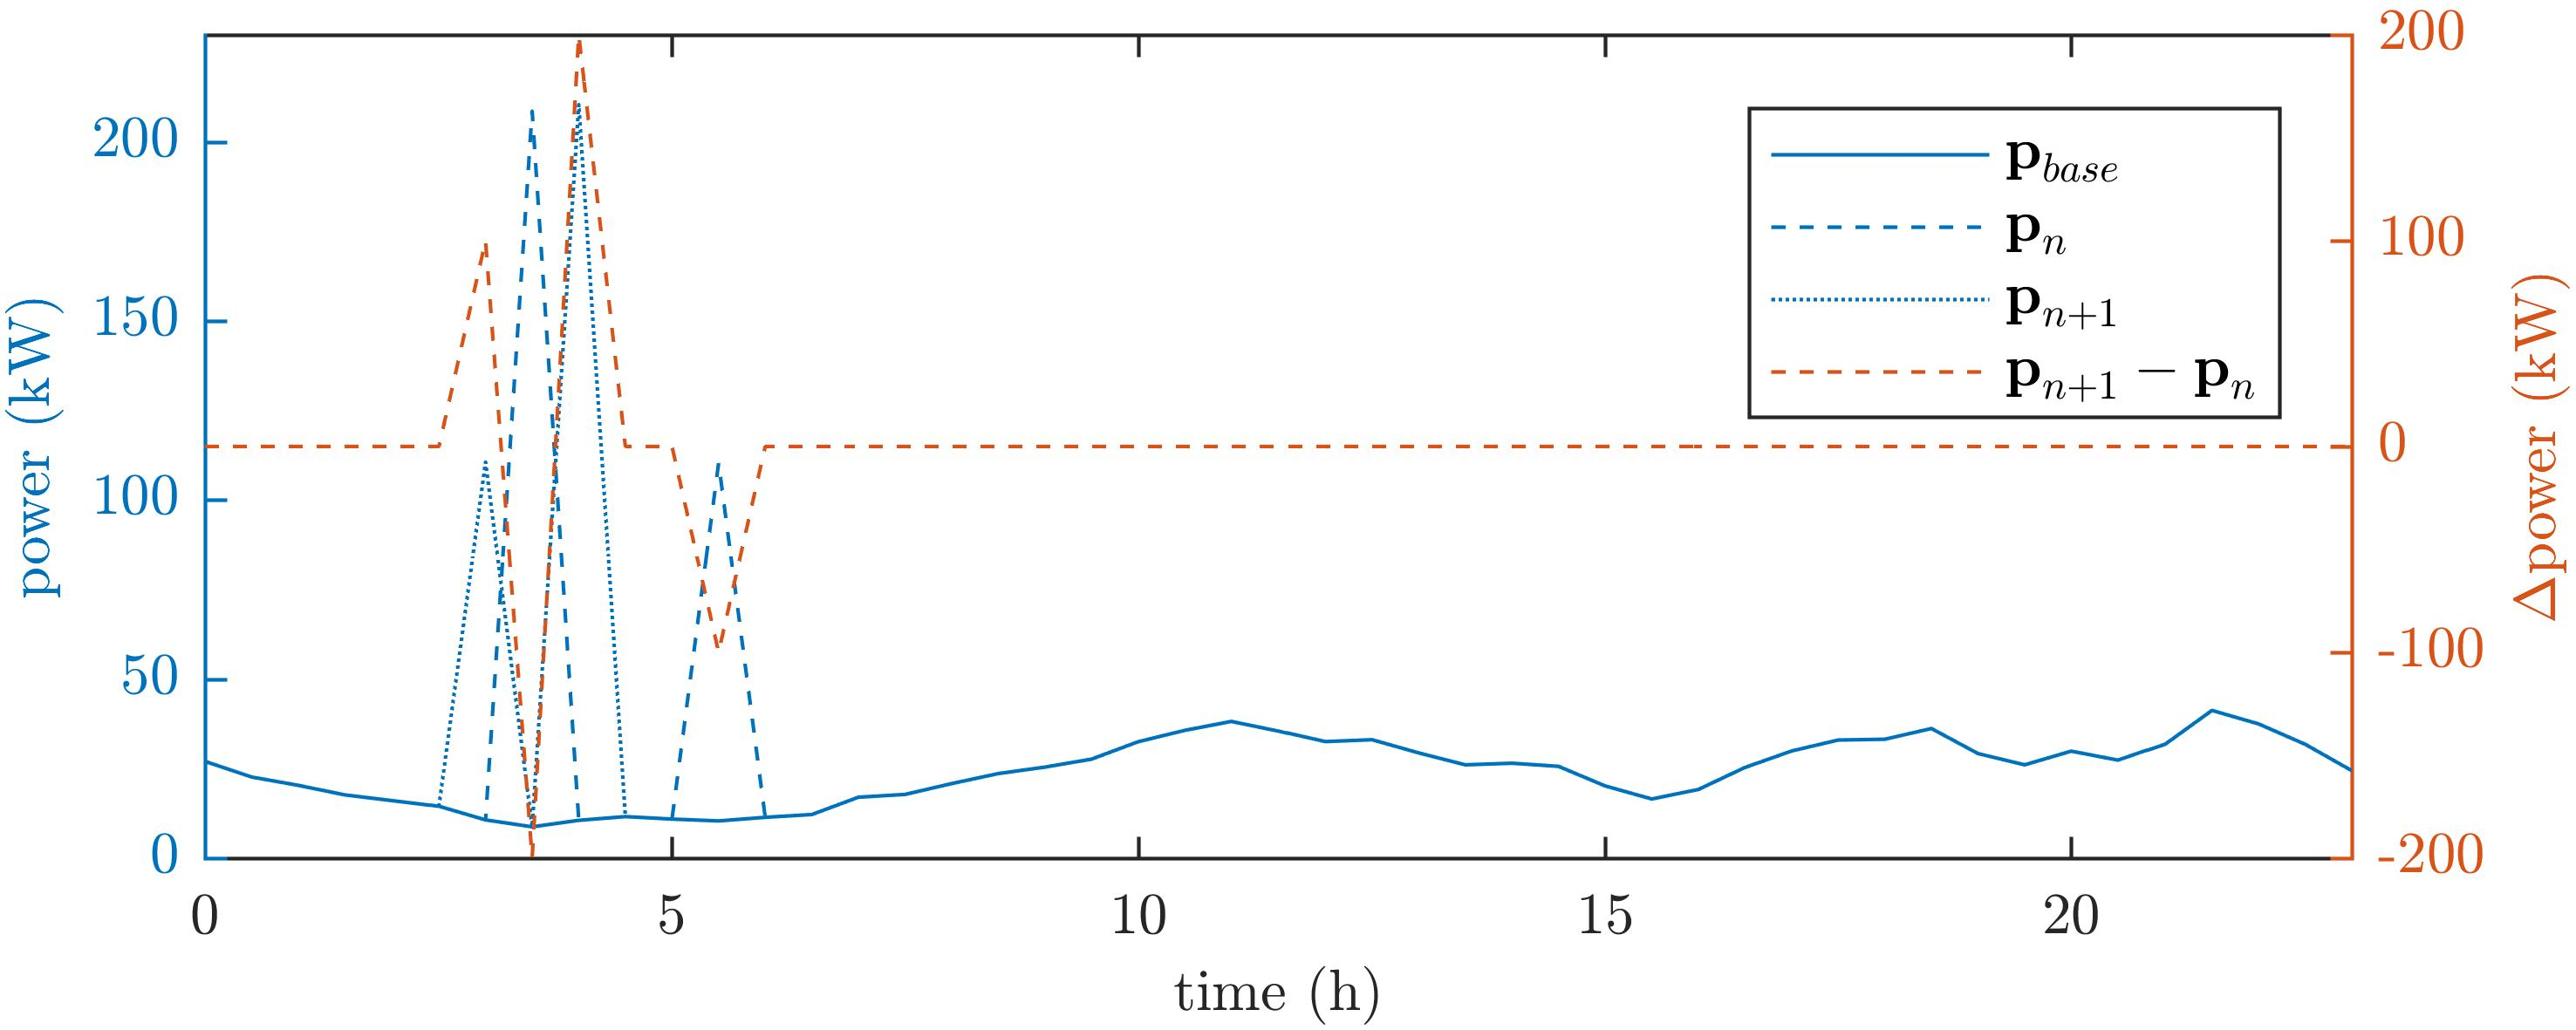
\includegraphics[height=4.5cm]{_chapter3/fig/oscillation/ts-i0100}
		\label{ch3:subfig:oscillation-last}
	}
\caption{Time series evolution for $\alpha=1.00$ and $\beta=1.00$, where (a) is at $n=1$, (b) is at $n=2$, (c) is at $n=3$, and (d) is at $n=N-1$.}
\label{ch3:fig:oscillation}
\end{figure}

\begin{table}\centering
	\begin{tabular}{r | C{2cm} C{2cm} | C{2cm} C{2cm}}
		\multirow{2}{*}{iteration ($n$)} & \multicolumn{2}{c|}{$\alpha=0.02$ and $\beta=0.20$} & \multicolumn{2}{c}{$\alpha=1.00$ and $\beta=1.00$} \\
	   & $\zeta_\text{PAR}$ & $\zeta_\text{TRA}$ & $\zeta_\text{PAR}$ & $\zeta_\text{TRA}$\\
	  	\hline
          1 & 46.84 & 45.86 & 46.84 & 45.86\\
          2 & 30.61 & 35.54 & 47.66 & 46.26\\
          3 & 20.10 & 27.31 & 46.84 & 45.86\\
          4 & 13.28 & 20.75 & 47.66 & 46.26\\
          5 & 8.83  & 15.56 & 46.84 & 45.86\\
          6 & 5.93  & 11.41 & 47.66 & 46.26\\
          7 & 4.02  & 8.20  & 46.84 & 45.86\\
          8 & 2.76  & 5.83  & 47.66 & 46.26\\
          9 & 1.92  & 4.24  & 46.84 & 45.86\\
         10 & 1.83  & 3.22  & 47.66 & 46.26\\
   $\vdots$ & $\vdots$ & $\vdots$ & $\vdots$ & $\vdots$\\
		100 & 1.83  & 2.72  & 47.66 & 46.26\\
   		\hline
   		\hline
   		convergence ($b$) & 0.47 & 0.32 & 0.00 & 0.00
	\end{tabular}
\sethlcolor{green}
	\caption{Comparison of $\zeta^\text{PAR}$ and $\zeta^\text{TRA}$ for two $\alpha$ and $\beta$ parameter pairs as shown in Figure~\ref{ch3:fig:oscillation} and Figure~\ref{ch3:fig:time-series}. Each value per iteration $n$ and the convergence $b$ is shown.}
	\label{ch3:tab:pair-comparison}
\end{table}

%  1 & 46.839871 & 45.855341 & 46.839871 & 45.855341\\
%  2 & 30.607134 & 35.537698 & 47.659842 & 46.257807\\
%  3 & 20.098148 & 27.310970 & 46.839871 & 45.855341\\
%  4 & 13.276370 & 20.747178 & 47.659842 & 46.257807\\
%  5 & 8.833609  & 15.564391 & 46.839871 & 45.855341\\
%  6 & 5.928785  & 11.409779 & 47.659842 & 46.257807\\
%  7 & 4.020532  & 8.204652  & 46.839871 & 45.855341\\
%  8 & 2.759917  & 5.831519  & 47.659842 & 46.257807\\
%  9 & 1.921657  & 4.239981  & 46.839871 & 45.855341\\
% 10 & 1.829655  & 3.223272  & 47.659842 & 46.257807\\
%100 & 1.829655  & 2.722986  & 47.659842 & 46.257807


Whereas the $\alpha$ and $\beta$ parameters use to produce the results in Figure~\ref{ch3:fig:time-series} reduced the power spike, those parameters in \ref{ch3:fig:oscillation} did not, where $\alpha = \beta = 1.0$.
In fact, an oscillating behaviour can be observed since the initially applied power profile is completely undone and completely reassigned onto a different demand trough.
Since this produces similar peaks, the same procedure repeats and reassigns the complete power profile back to the original demand troughs.
In the end, these charging spikes could never be fully mitigated and the algorithm did not smoothen the total demand.
This issue becomes more evident when comparing the $\zeta_\text{PAR}$ and $\zeta_\text{TRA}$ values are compared for both parameter pairs.
The evolution of $\zeta_\text{PAR}$ and $\zeta_\text{TRA}$, as tabulated in Table \ref{ch3:tab:pair-comparison}, shows this difference in performance and convergence of the algorithm when subjected to different values of $\alpha$ and $\beta$.
Therefore, multiple parameter pairs across the entire range of $\alpha$ and $\beta$ are studied to determine how the algorithm performs for each given pair.
The results for the synchronised algorithm performance are plotted in Figure~\ref{ch3:fig:all-sync}.

\begin{figure}\centering
	\subfloat[]{
		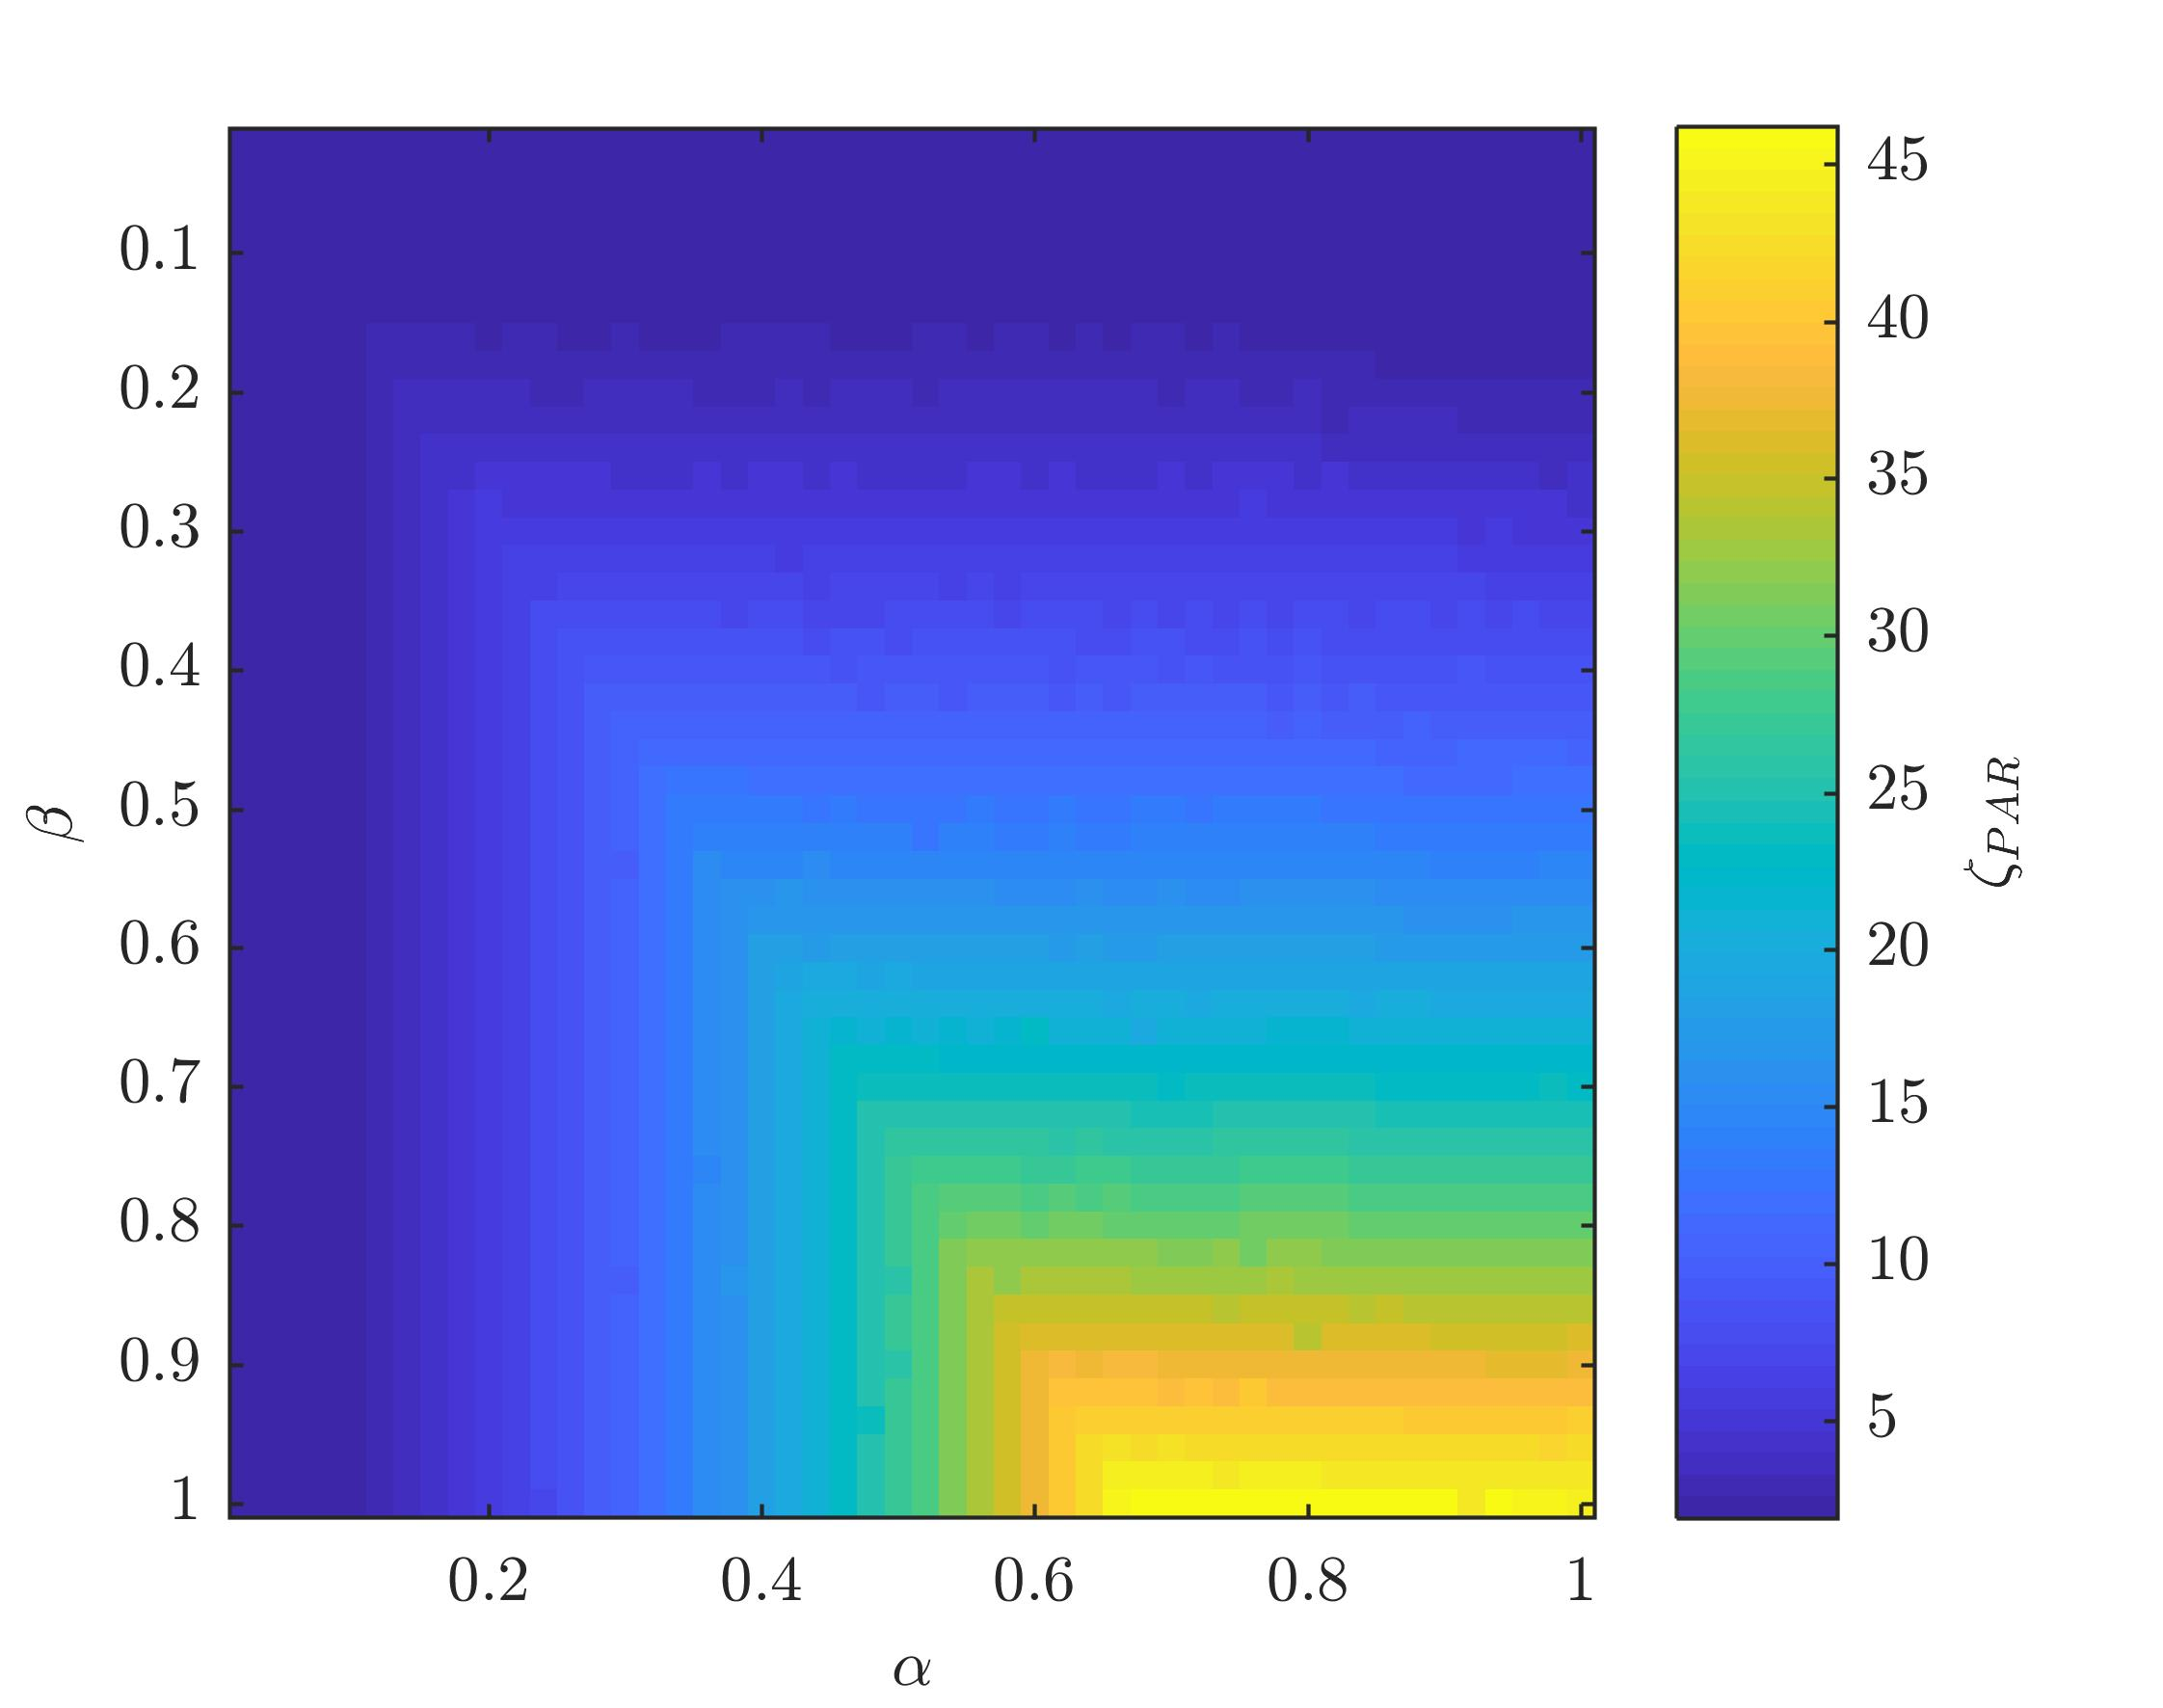
\includegraphics[width=0.5\linewidth]{_chapter3/fig/all-sync/3-all_par}
		\label{ch3:subfig:all-sync-par}
	}
	\subfloat[]{
		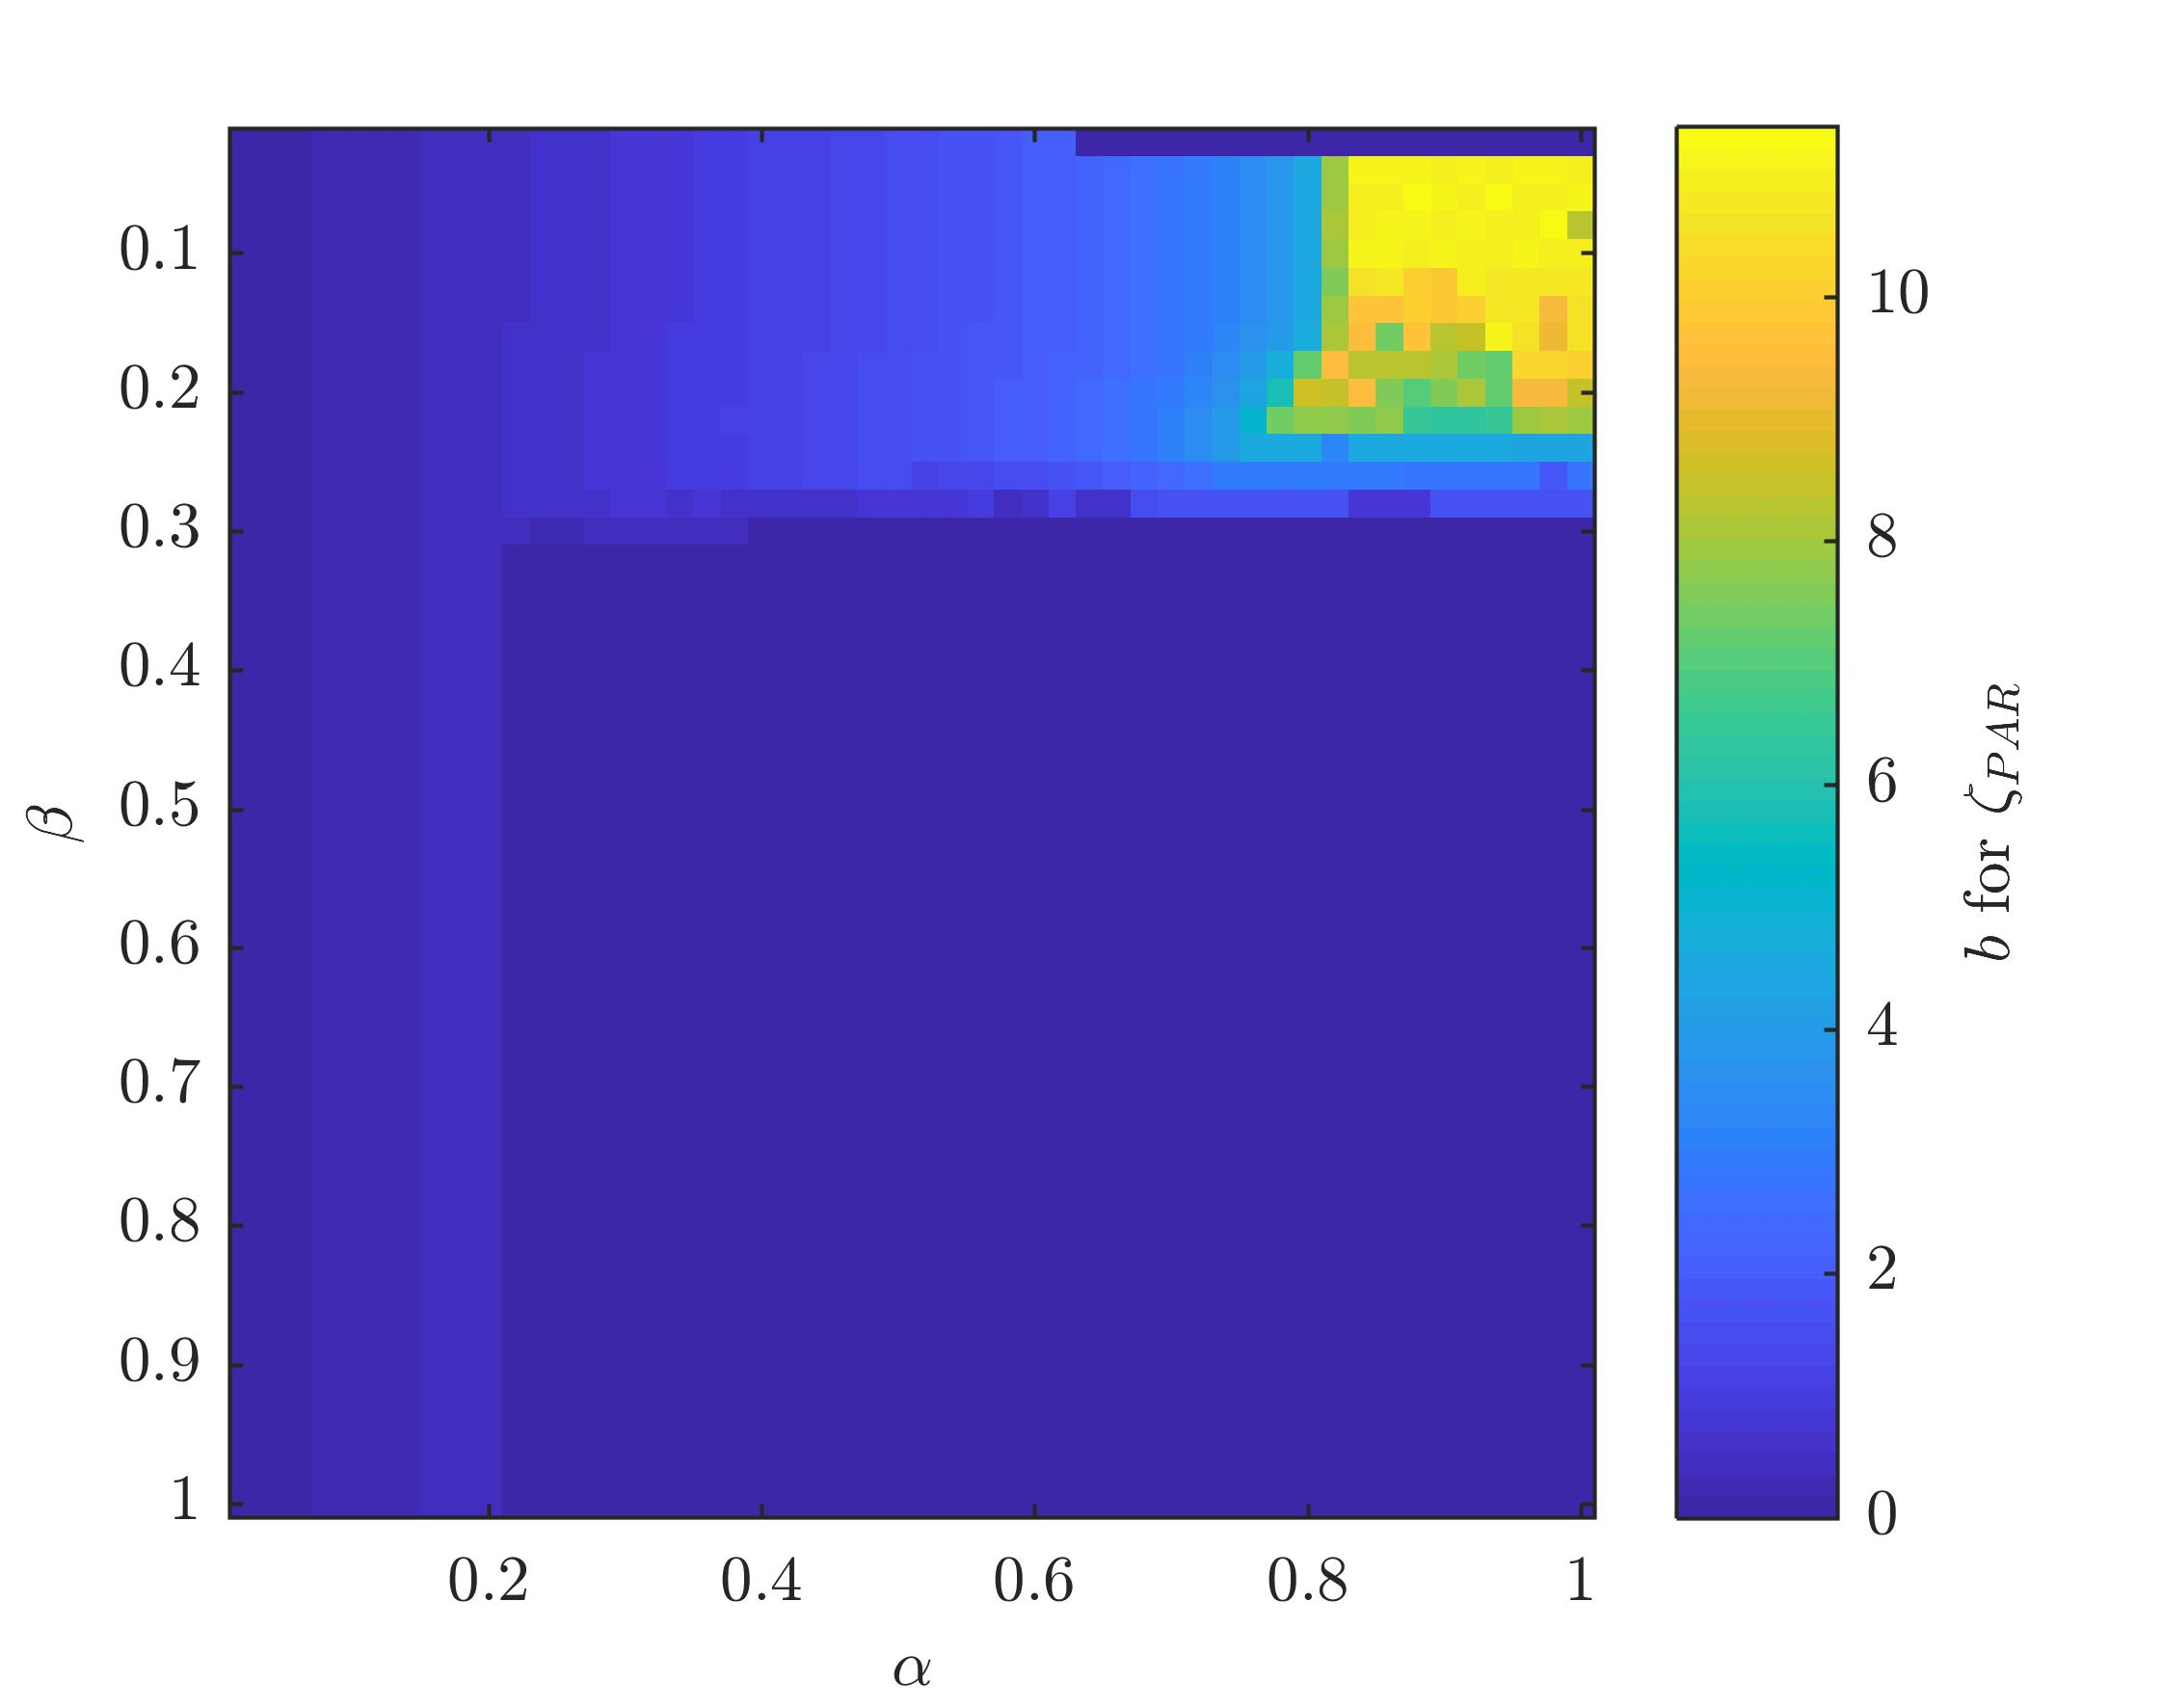
\includegraphics[width=0.5\linewidth]{_chapter3/fig/all-sync/3-all_par_conv}
		\label{ch3:subfig:all-sync-par-conv}
	}\\
	\subfloat[]{
		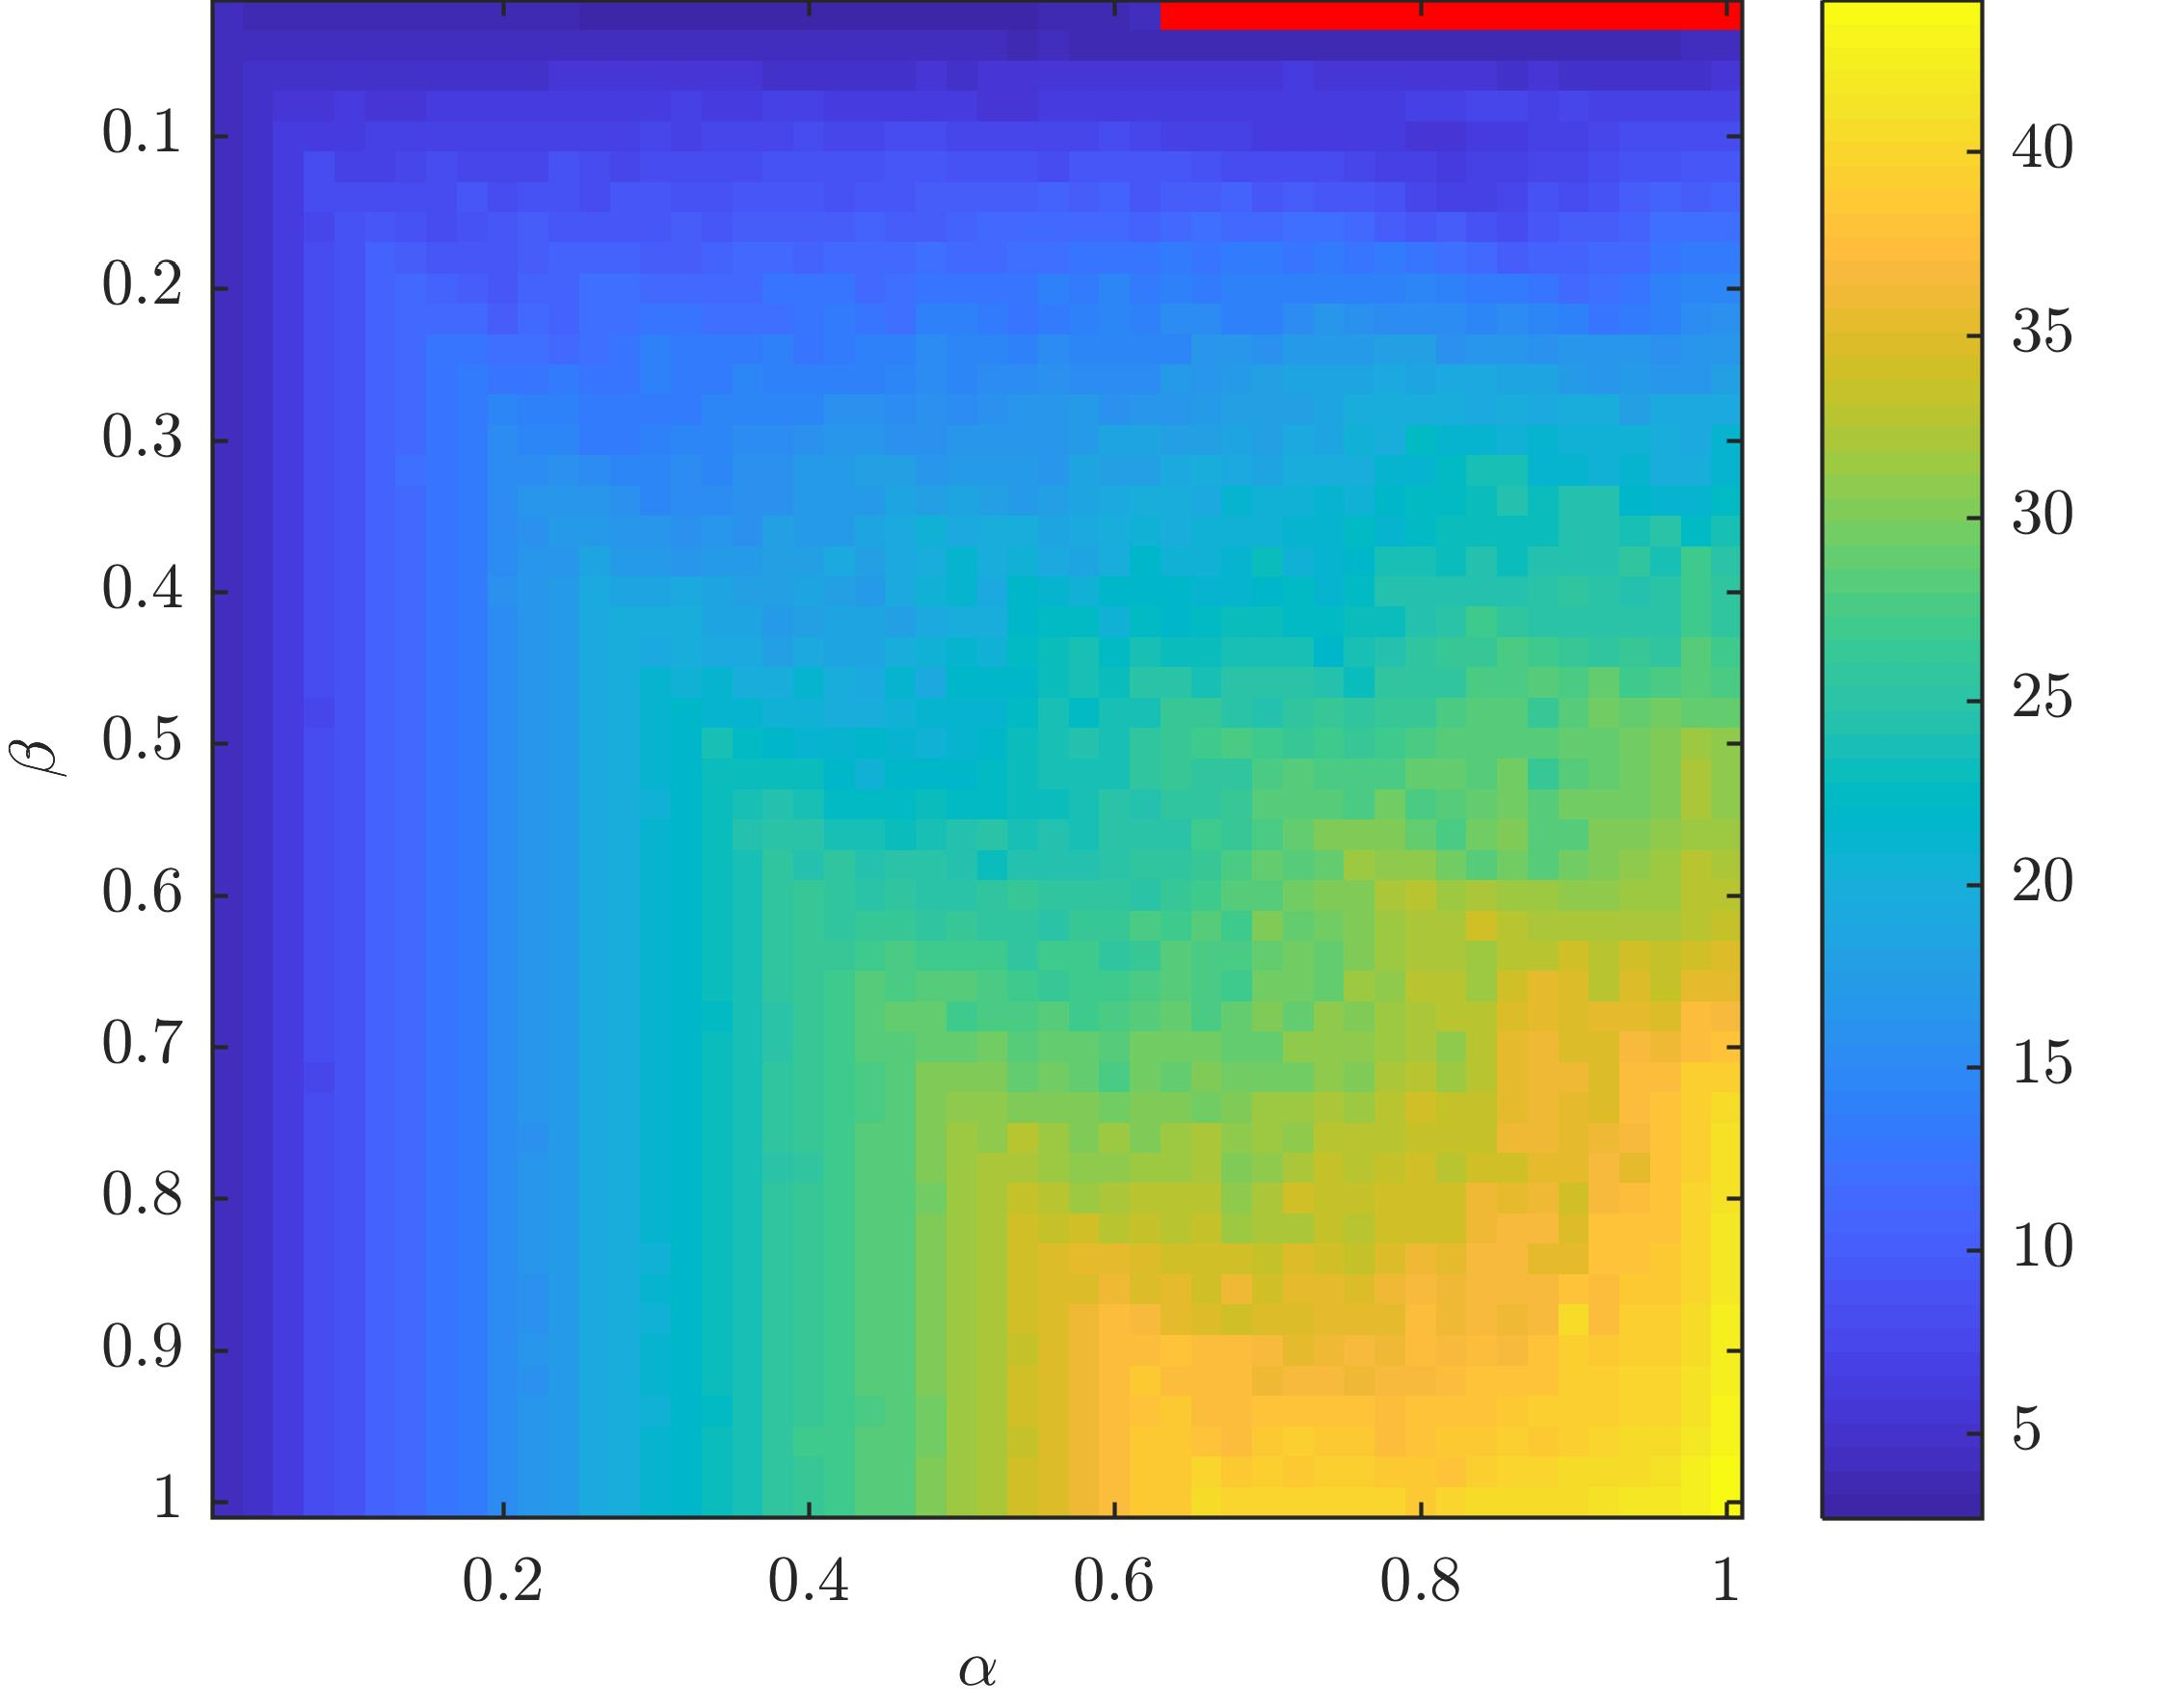
\includegraphics[width=0.5\linewidth]{_chapter3/fig/all-sync/3-all_tra}
		\label{ch3:subfig:all-sync-tra}
	}
	\subfloat[]{
		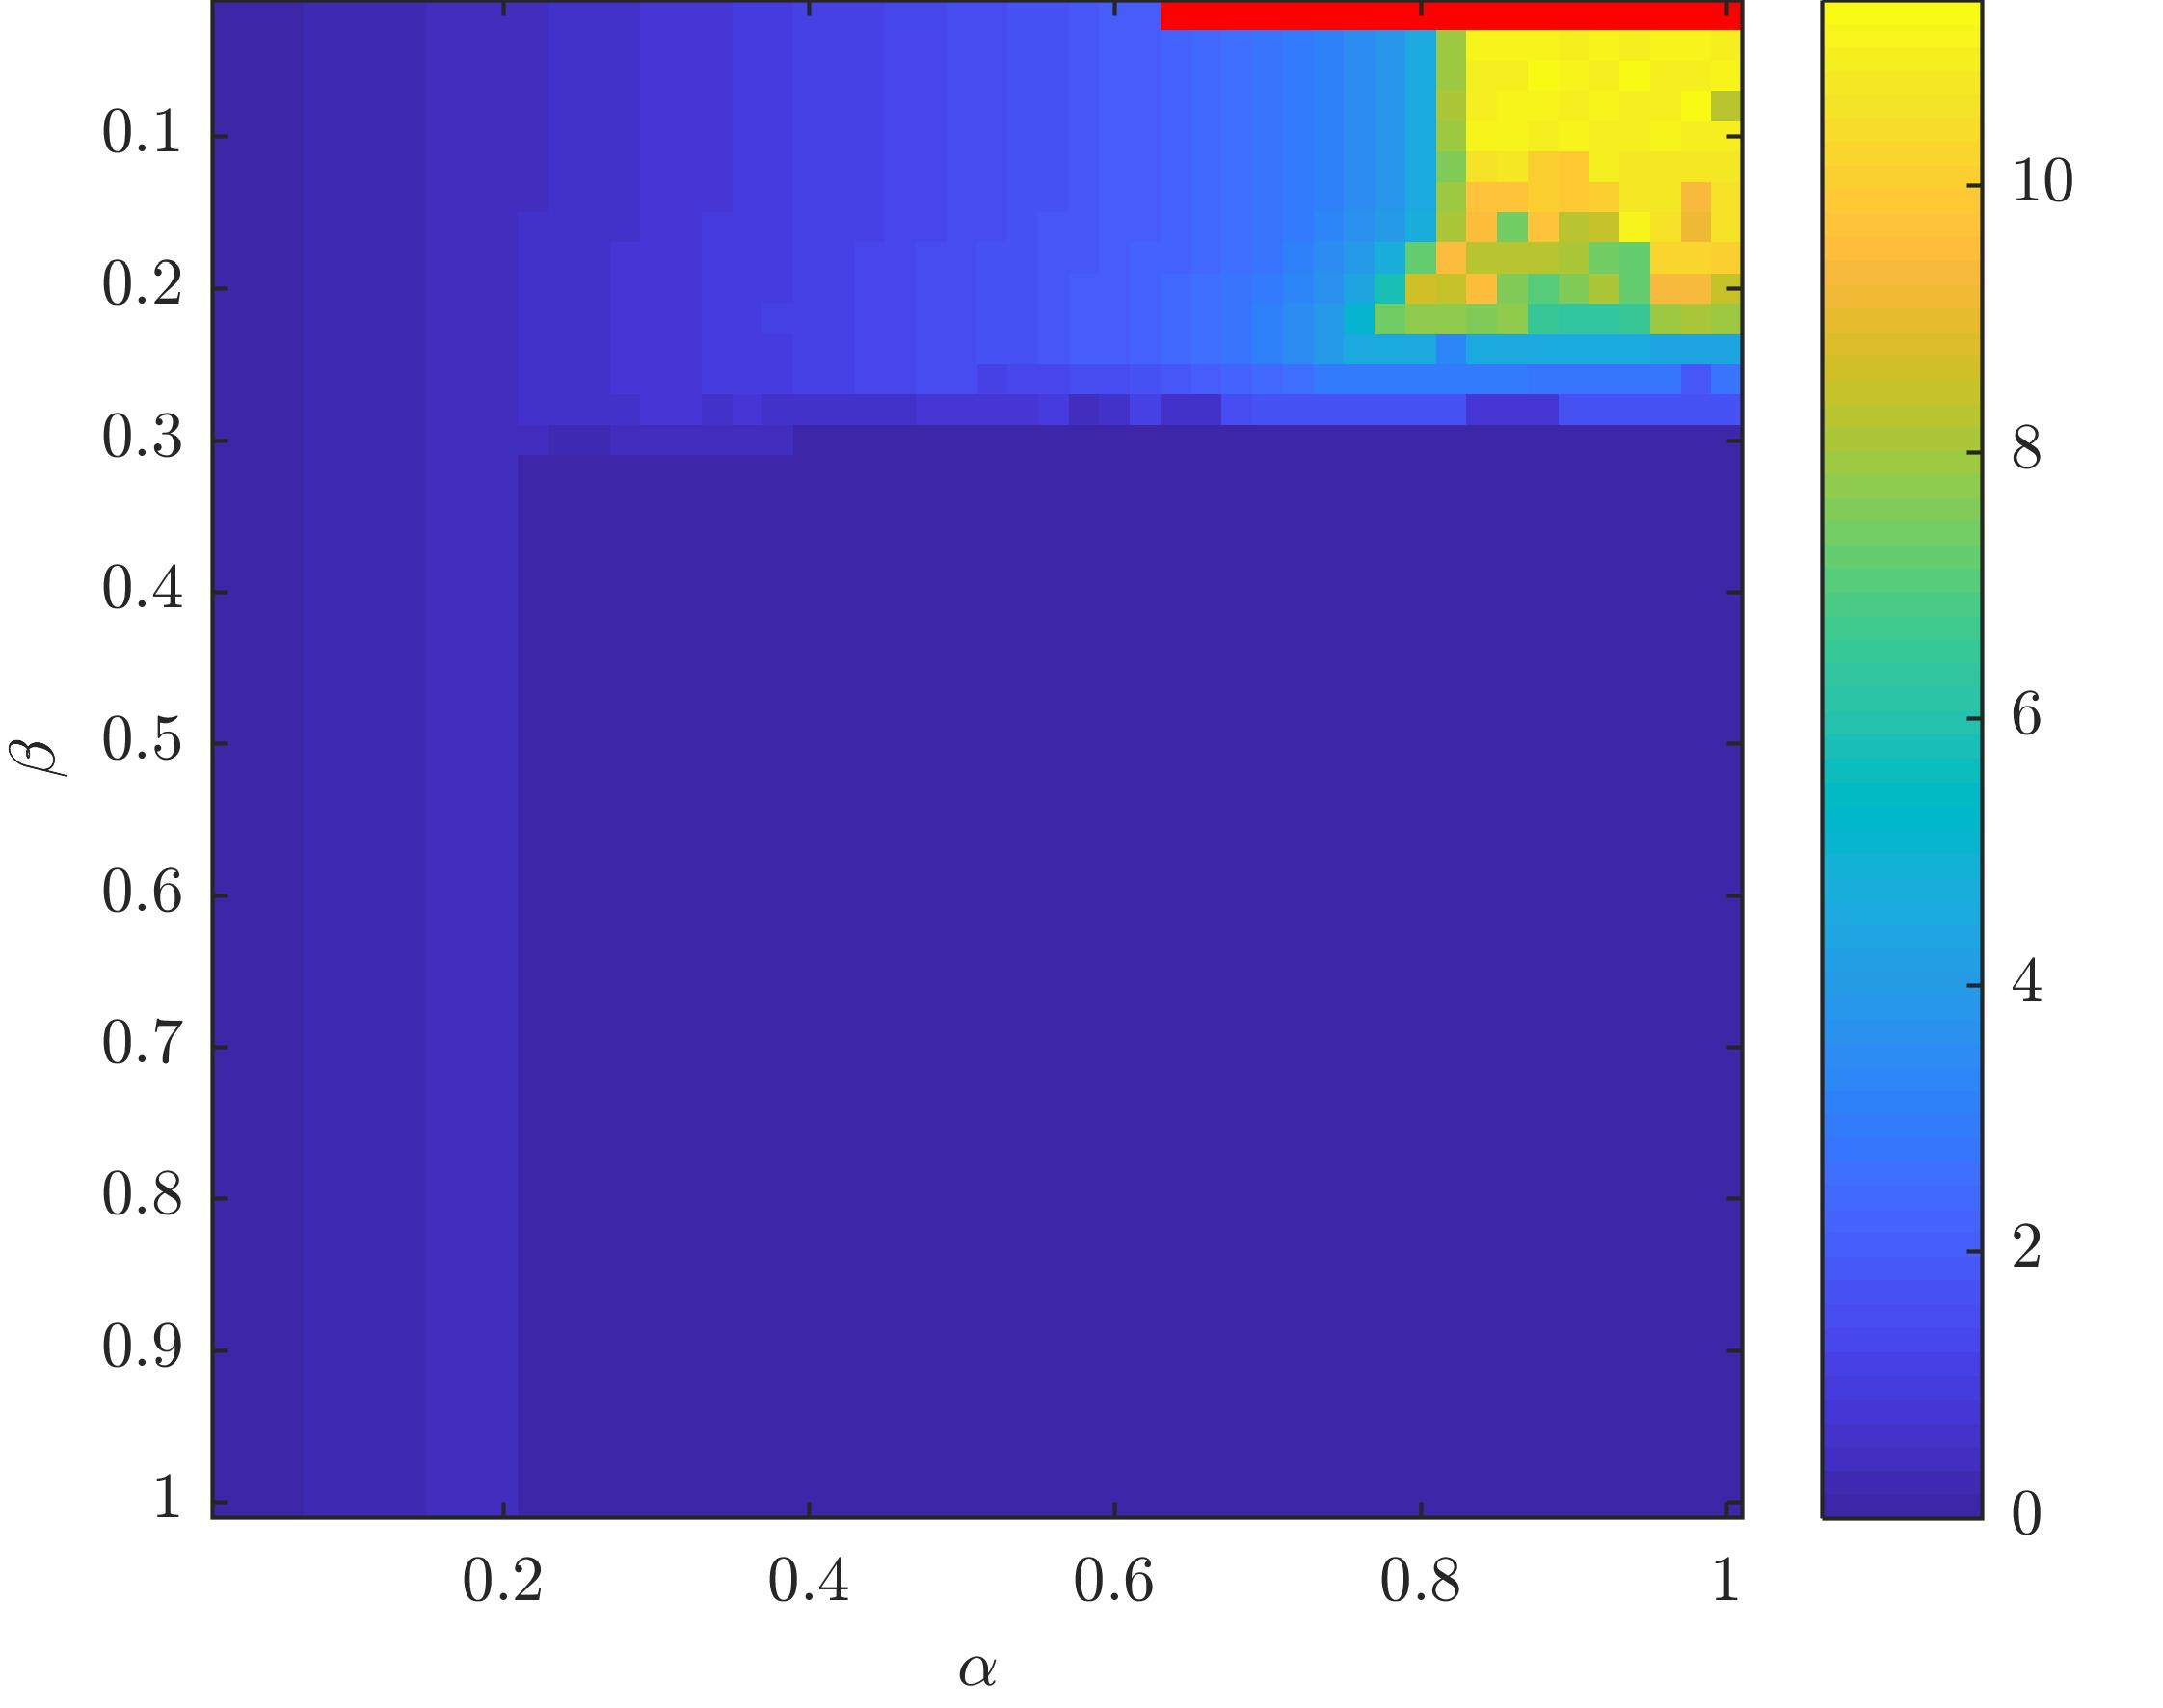
\includegraphics[width=0.5\linewidth]{_chapter3/fig/all-sync/3-all_tra_conv}
		\label{ch3:subfig:all-sync-tra-conv}
	}\\
	\caption{Full range analysis of $\alpha$ and $\beta$ where, (a) shows the final $\zeta_\text{PAR}$, (b) shows the convergence, $b$, for $\zeta_\text{PAR}$, (c) shows the final $\zeta_\text{TRA}$, and (d) shows the convergence, $b$, for $\zeta_\text{TRA}$ (red indicates missing data).}
	\label{ch3:fig:all-sync}
\end{figure}

Figure~\ref{ch3:subfig:all-sync-par} and Figure~\ref{ch3:subfig:all-sync-tra} show how the final values for both $\zeta_\text{PAR}$ and $\zeta_\text{TRA}$ were lowest when either $\alpha$ or $\beta$ was chosen closer to zero.
This result coincides with the finding that hard reduction and reallocation lead to an oscillating behaviour of the algorithm.
Similarly, the convergence of those two performance metrics, as shown in Figure~\ref{ch3:subfig:all-sync-par-conv} and Figure~\ref{ch3:subfig:all-sync-tra-conv}, was best when $\alpha$ approached one and $\beta$ approached zero.
This behaviour is by design, since a larger value of $\alpha$ increases the rate at which the currently applied peak is reduced, whilst a smaller value of $\beta$ limits the amount that can be reallocated for each time slot.
Such clear behavioural differences for different pairs of $\alpha$ and $\beta$ indicate an optimal operation region of the algorithm within the north-east quadrant of the plot.
Whether this behaviour is till observed, and the question whether the algorithm still performs when introducing desynchronisation, is answered in the subsequent section, Section~\ref{ch3:subsec:algorithm-performance-desynchronised-regular}.


\subsection{Algorithm performance for desynchronised operation - regular timing}
\label{ch3:subsec:algorithm-performance-desynchronised-regular}

\begin{figure}\centering
	\subfloat[]{
		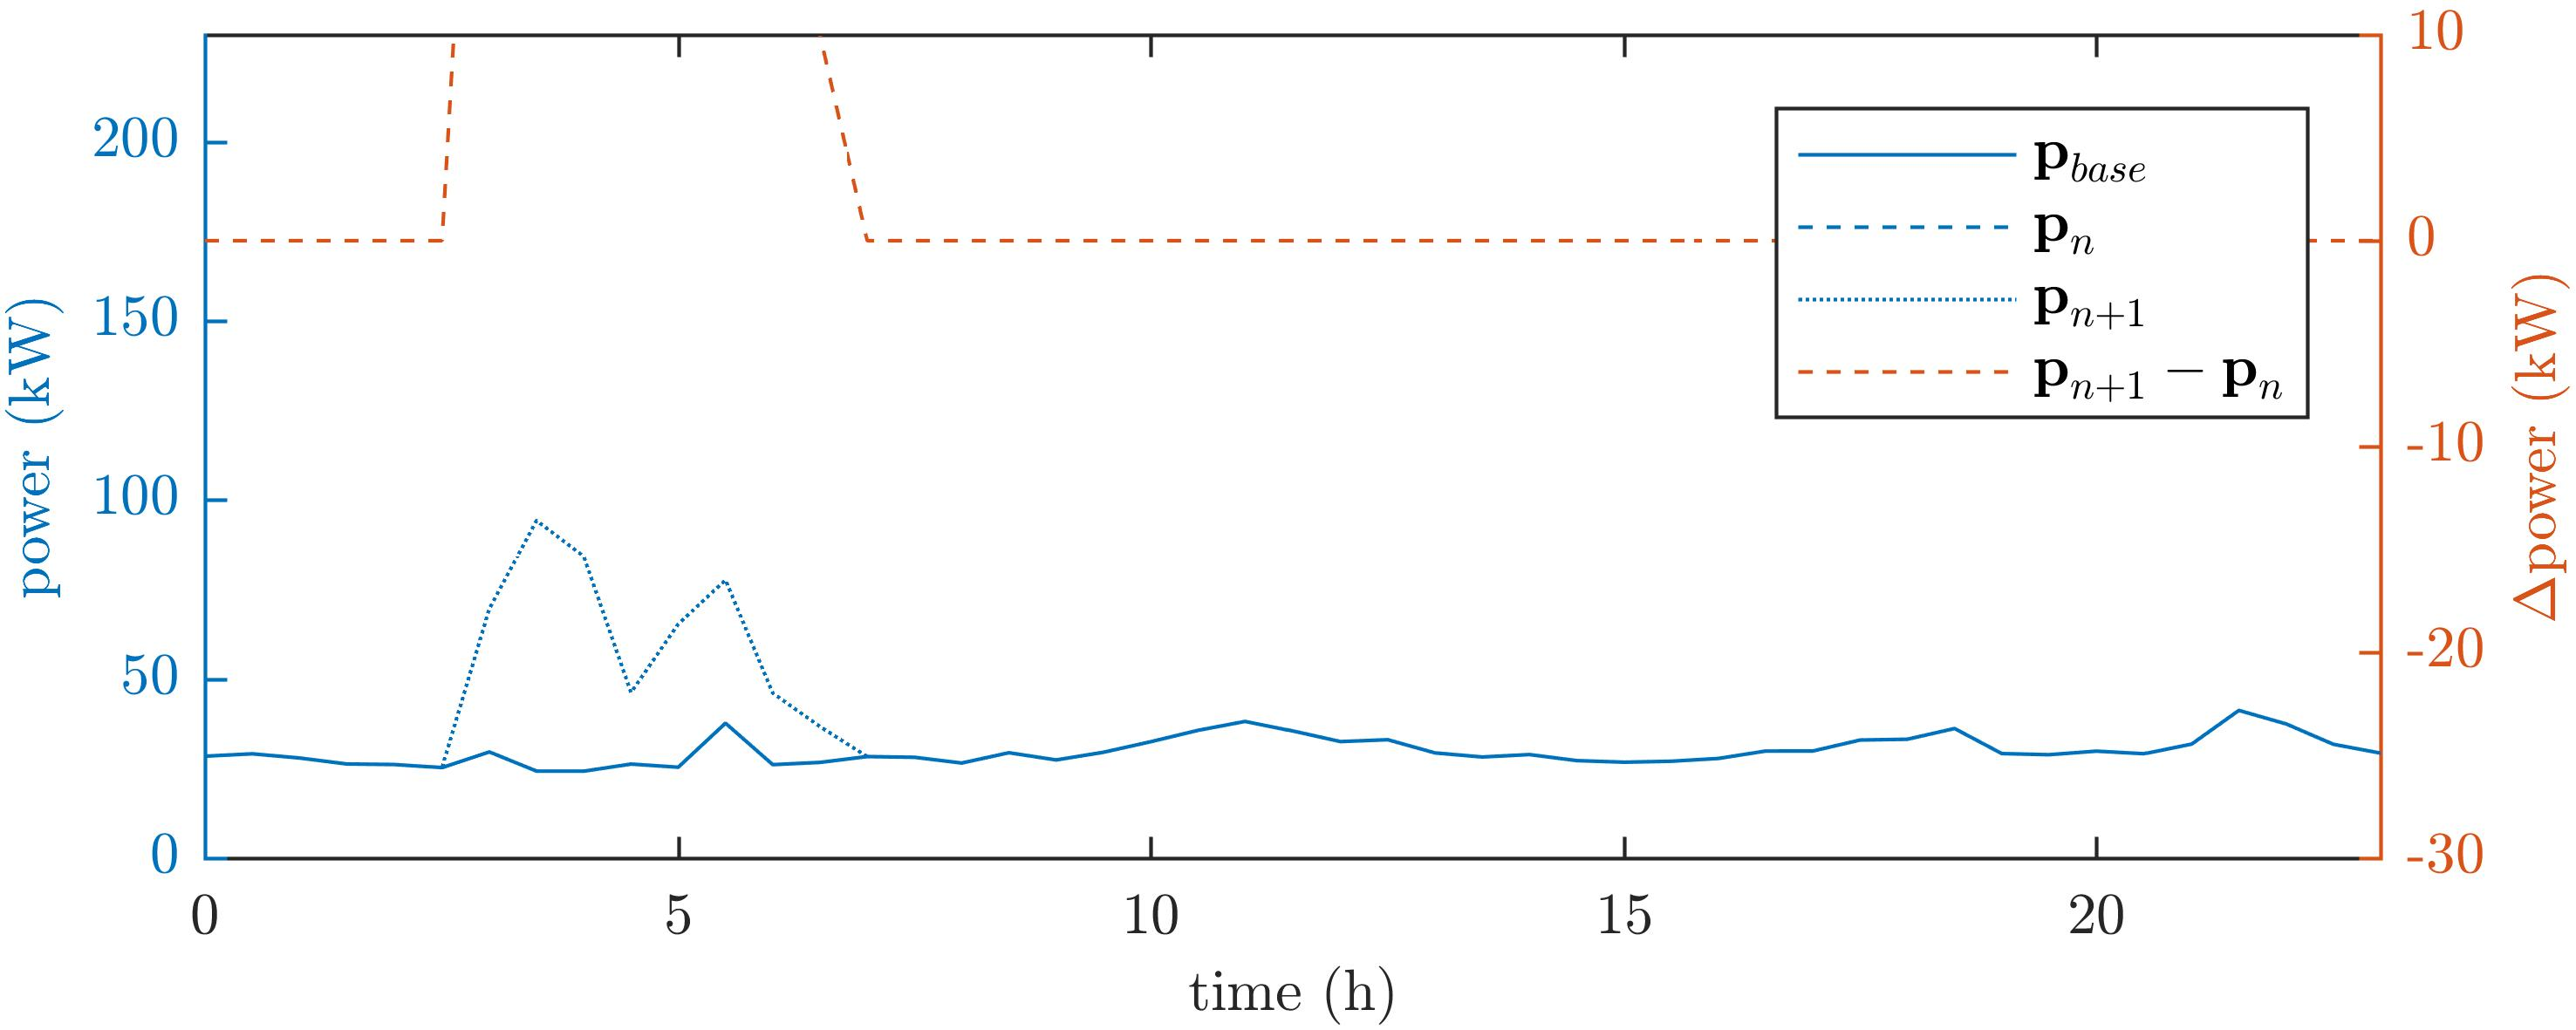
\includegraphics{_chapter3/fig/time-series-desync/as-r-ts-i0001}
		\label{ch3:subfig:time-series-desync-1}
	}\\
	\subfloat[]{
		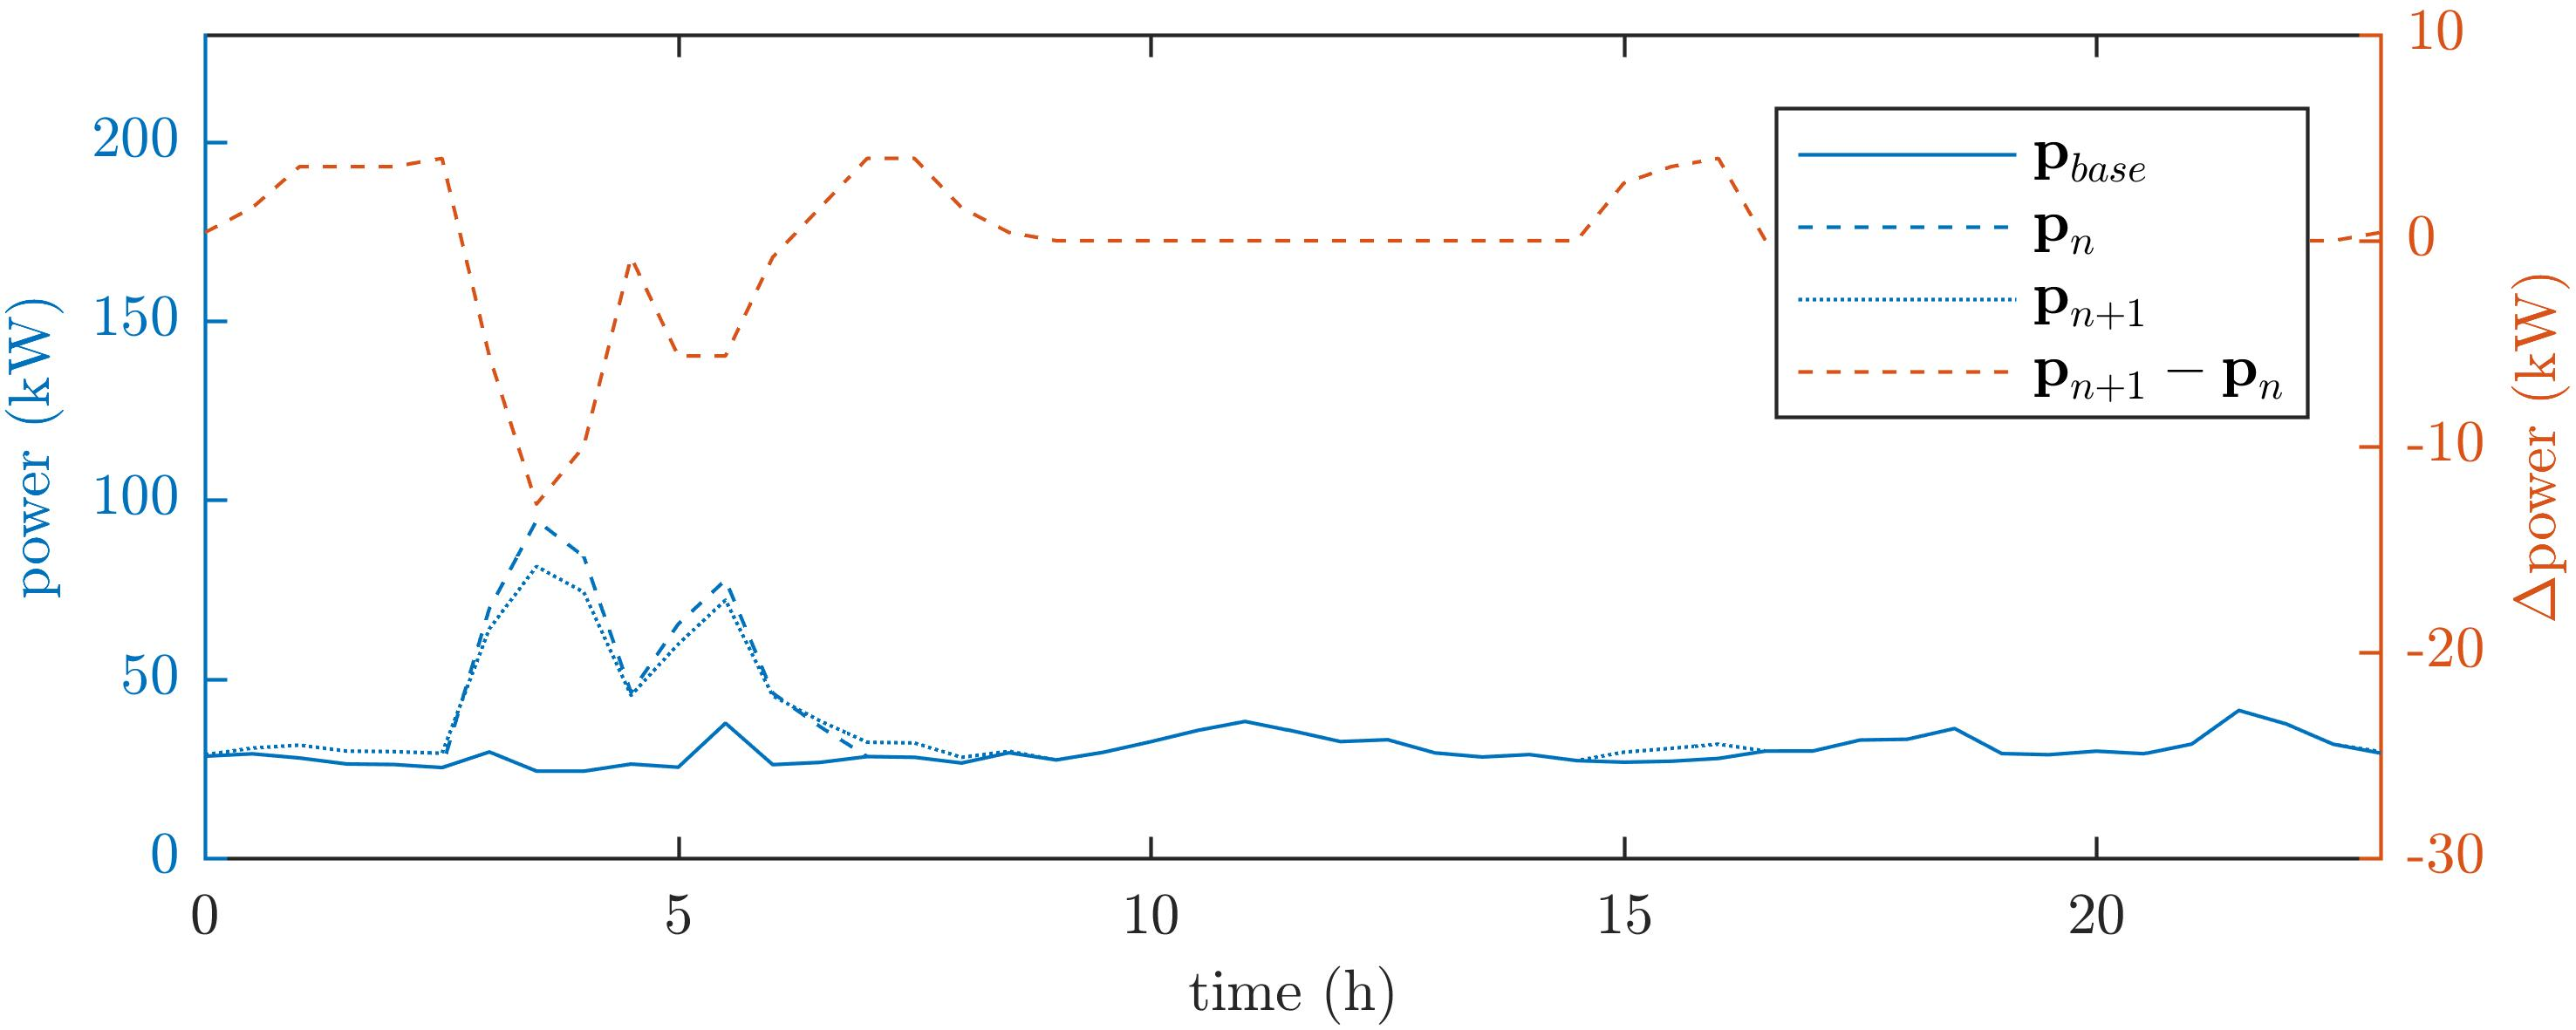
\includegraphics{_chapter3/fig/time-series-desync/as-r-ts-i0002}
		\label{ch3:subfig:time-series-desync-2}
	}\\
	\subfloat[]{
		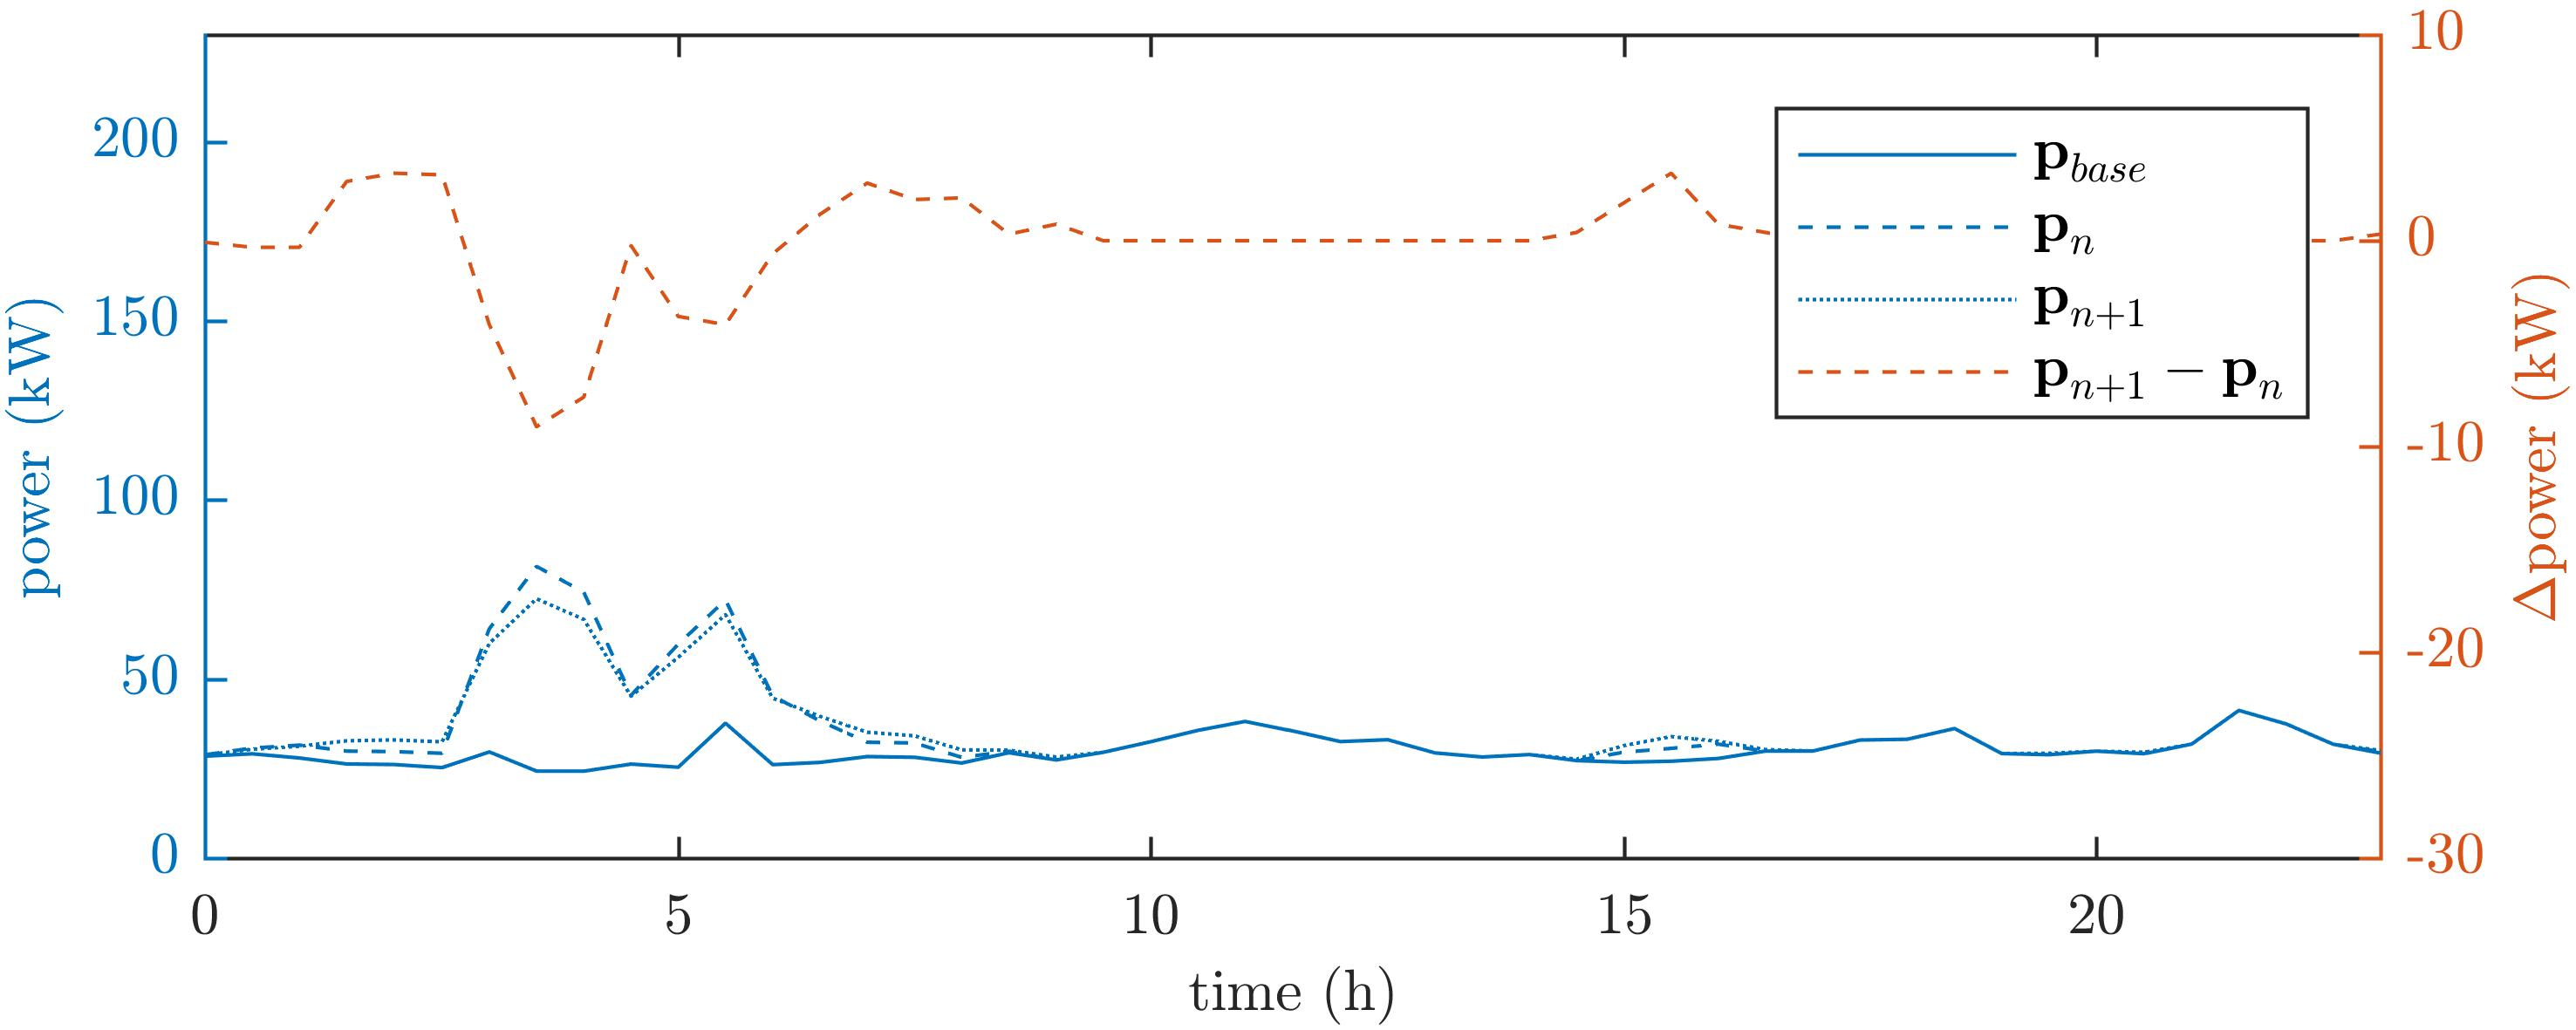
\includegraphics{_chapter3/fig/time-series-desync/as-r-ts-i0003}
		\label{ch3:subfig:time-series-desync-3}
	}\\
	\subfloat[]{
		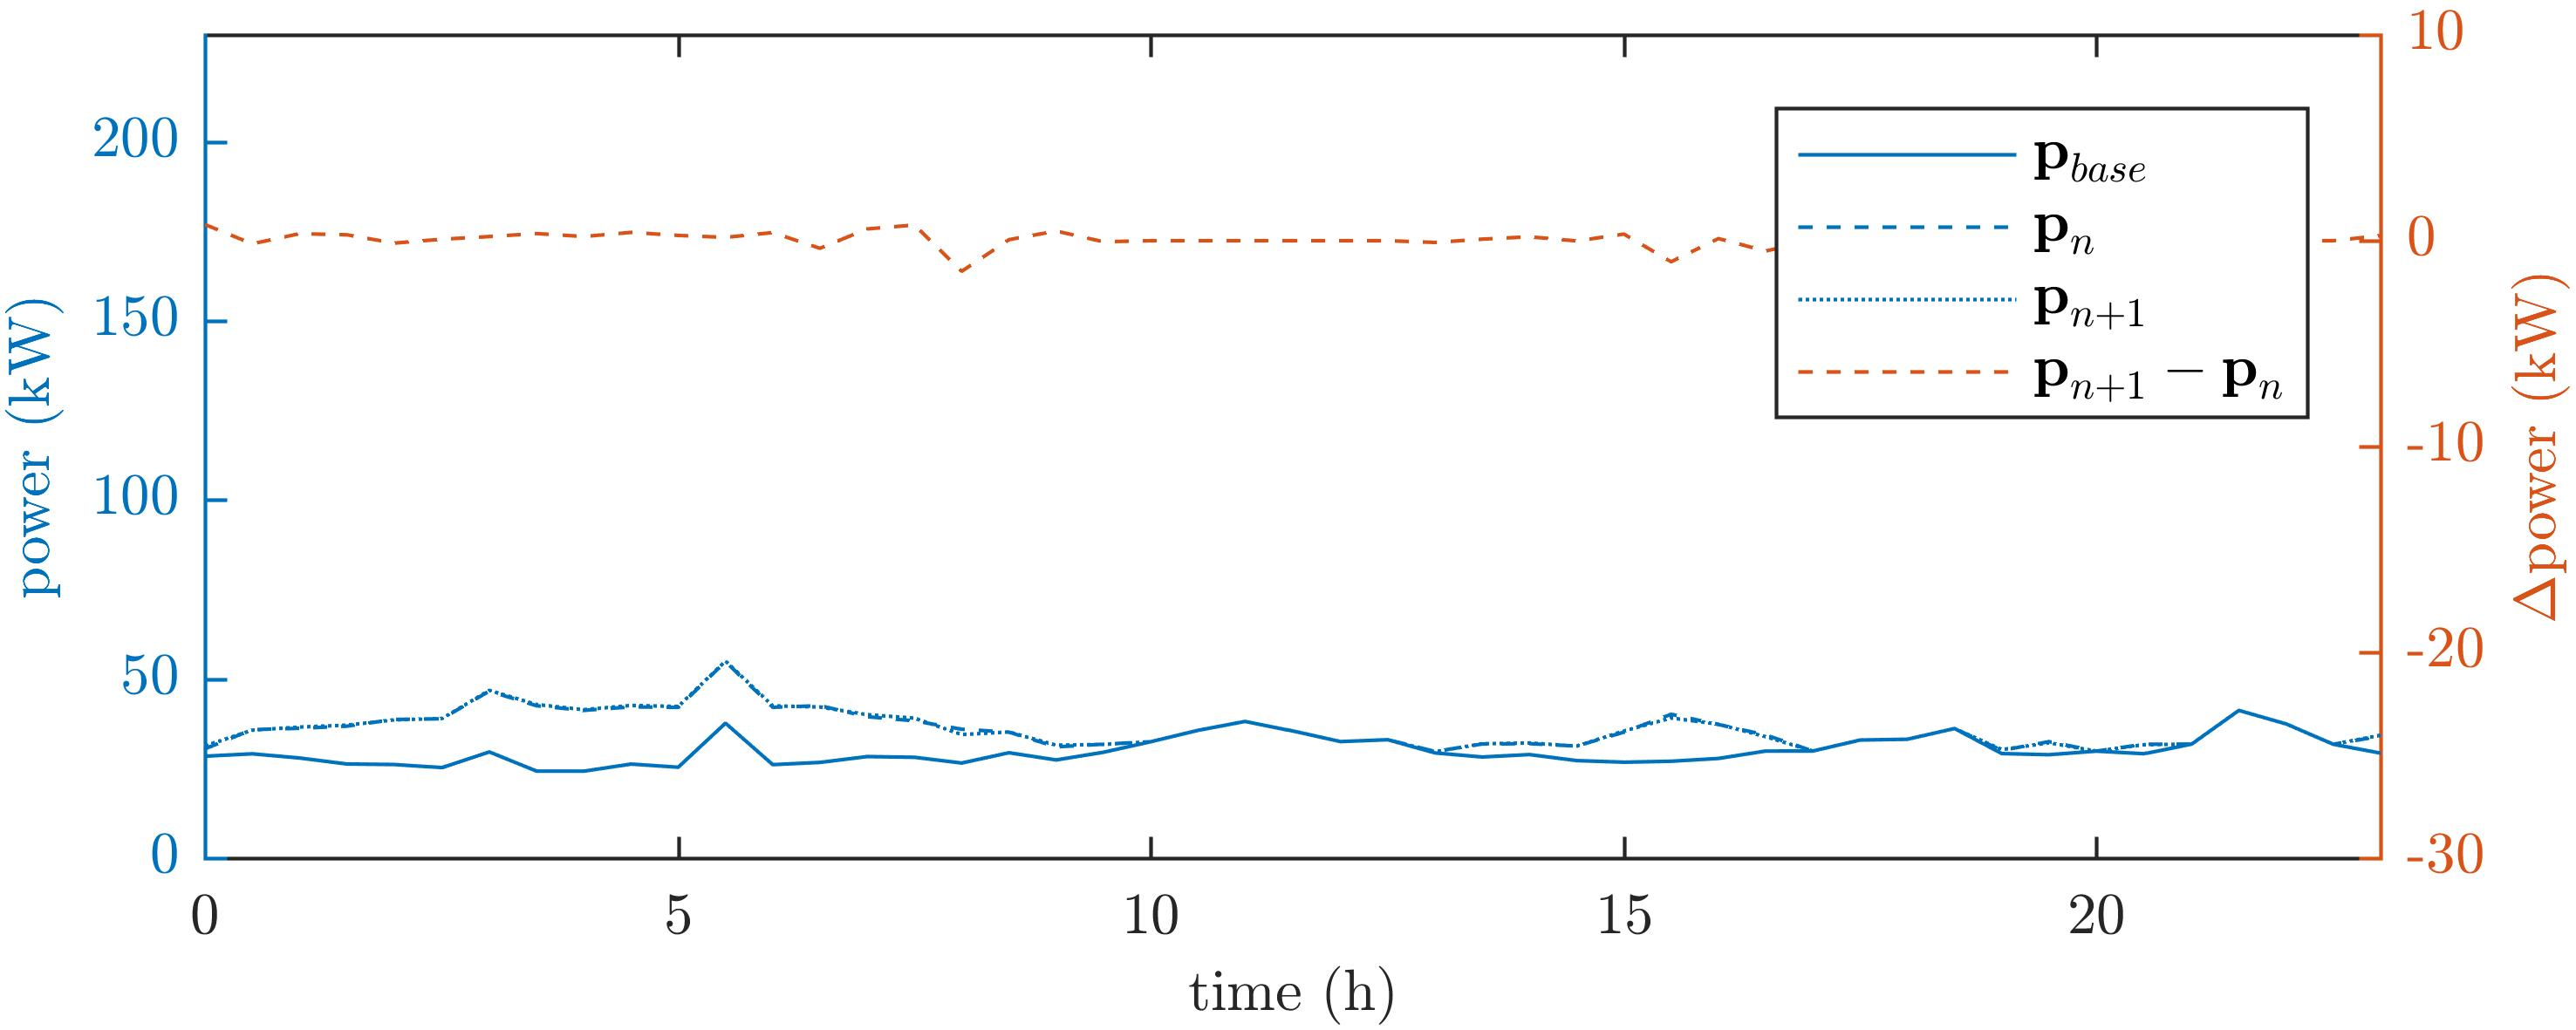
\includegraphics{_chapter3/fig/time-series-desync/as-r-ts-i0100}
		\label{ch3:subfig:time-series-desync-last}
	}
	\caption{Desynchronised time series evolution for $\alpha=0.02$ and $\beta=0.20$, where (a) is at $n=1$, (b) is at $n=2$, (c) is at $n=3$, and (d) is at $n=N-1$.}
	\label{ch3:fig:time-series-desync}
\end{figure}

Looking at the evolution of the time-series when desynchronising the algorithm's execution shows significant differences already.
Figure~\ref{ch3:fig:time-series-desync} shows this evolution for the same parameters as those chosen for Figure~\ref{ch3:fig:time-series}.
The difference is however, that the assignment of charging powers lead to a significantly lower demand spike at the very beginning of executing the algorithm.
Subsequent iterations then reduce this spike much broader than it has been the case when executing the algorithm in a synchronised manner.

\subsection{Algorithm performance for desynchronised operation - irregular timing}
\label{ch3:subsec:algorithm-performance-desynchronised-irregular}
